\section{Identifying Opportunities to Decide\label{sec:dilemma-trilemma}}
% Previously titled
% Every Bureaucrat's  Dilemmas

% Not included here: 
% https://en.wikipedia.org/wiki/The_Innovator%27s_Dilemma
% because it is the etic view of change

% This .tex file contains a GraphViz diagram of the relations
% between dilemmas and recurring themes.
% Each line of GraphViz source code begins with "%GV". For example,
%GV digraph G {
%GV // from the bureaucracy book dilemmas_and_trilemmas.text
%GV // https://dreampuf.github.io/GraphvizOnline
%GV rankdir=LR;

Bureaucracy is the set of subjective decisions people make as part of an effort to manage resources shared by a community. 
%This definition applies from the outsiders perspective (organizations responsible for shared resources are bureaucratic) and internal to the organization (bureaucrat members negotiate with other members of the organization)
Bureaucrats face a multitude of decisions independent of the specific shared resource and independent of which organization the bureaucrat is a member of. To build your process empathy, in this section I review decisions you will face as a bureaucrat.

When a decision has two viable options (neither being best), that is a \href{https://en.wikipedia.org/wiki/Dilemma}{dilemma}. 
\index{Wikipedia!dilemma@\href{https://en.wikipedia.org/wiki/Dilemma}{dilemma}}\iftoggle{WPinmargin}{\marginpar{$>$Wikipedia: dilemma}}{}
The name for a decision with three viable options is a \href{https://en.wikipedia.org/wiki/Trilemma}{trilemma}. 
\index{Wikipedia!trilemma@\href{https://en.wikipedia.org/wiki/Trilemma}{trilemma}}
This section describes a bureaucrat's experience of operating within an organization in terms of dilemmas and trilemmas. Instead of focusing on moral dilemmas~\cite{2017_Zacka} or institutional ethics, here I focus on interpersonal relationships and the logistics of allocating your attention. 

%Dilemma are not unique to bureaucracy. 
Dilemmas are a \href{https://en.wikipedia.org/wiki/Defeasible_reasoning}{simple way}
\index{Wikipedia!defeasible reasoning@\href{https://en.wikipedia.org/wiki/Defeasible_reasoning}{defeasible reasoning}}\iftoggle{WPinmargin}{\marginpar{$>$Wikipedia: Defeasible\\reasoning}}{}
of discussing decisions. % but are not the only relevant aspect of bureaucracy.
Dilemmas are a useful framing to highlight the following concepts:
\begin{itemize}
    \item You, an individual bureaucrat, face decisions that you may not have recognized. Failing to recognize a choice (an error by omission\footnote{The other category of error is error by commission -- you recognized the need to select among options but made the wrong decision.}) can lead to suboptimal results. The dilemmas below are generic to any bureaucratic process and are intended to stimulate your ability to identify decisions. 
    \item You face complex trade-offs in your role as a bureaucrat. Dilemmas are intended as an entry point to more nuanced reflection that is specific to your situation. The dilemmas below are not exhaustive; this list is merely illustrative. 
    \item You can use dilemmas as an entry to \href{https://en.wikipedia.org/wiki/Theory_of_mind}{intellectual empathy} 
    \index{Wikipedia!Theory of mind@\href{https://en.wikipedia.org/wiki/Theory_of_mind}{Theory of Mind}}\iftoggle{WPinmargin}{\marginpar{$>$Wikipedia: Theory\\of mind}}{}
    with fellow bureaucrats when you recognize they face the same dilemmas. These dilemmas are generic to the situation and the person facing the decisions. You now have a topic to discuss with them. You can share your understanding. 
    \item You can be curious about the choice other bureaucrats select for a given dilemma. Everyone in the organization faces these decisions, so these dilemmas give you a topic of conversation to better understand each bureaucrat's view.
    \item When you encounter a bureaucratic process that does not feel intuitive, 
    you can try to understand which dilemmas the designers faced. 
    You need to identify relevant dilemmas to build \gls{process empathy}. \iftoggle{glossaryinmargin}{\marginpar{[Glossary]}}{}
    \item You can identify and negotiate potential sources of friction. Other bureaucrats may arrive at different selections for a given dilemma, so recognizing this and discussing it can improve the effectiveness of all involved.
    \item If you don't recognize the existence of the dilemmas or name them, bureaucracy can feel like resistance, confusion, conflict, and frustration. By recognizing the dilemmas specific to your situation, you can see that bureaucracy is  a set of opportunities and potential disagreements that can be negotiated.
\end{itemize}


% claim
Dilemmas explain the inherent complexity of bureaucracy even when bureaucrats are honest and the purpose of the organization is clear.
% relevance
The point isn't that one should \href{https://en.wikipedia.org/wiki/False_dilemma}{select one of the two options}. 
\index{Wikipedia!false dilemma@\href{https://en.wikipedia.org/wiki/False_dilemma}{false dilemma}}\iftoggle{WPinmargin}{\marginpar{$>$Wikipedia: False\\dilemma}}{}
The point of recognizing a dilemma is that it is a marker that there is a decision to be made.
% consequence
Once the need for a decision is identified, the action for the bureaucrat is not to select one of the two options. The effective bureaucrat identifies nuances, enumerates alternatives, and talks with fellow bureaucrats about these decisions. Rather than seeking consensus, strive for comprehension of other people's perspectives. That way you can navigate decision-making processes more effectively.

The choices described below in the simplified representation of dilemmas are intended as a starting point for introducing the decision space relevant to individual bureaucrats. Do not accept the dilemmas presented here as the final framing. Thinking in terms of a limited spectrum of opportunities neglects nuances that enable more creative approaches. 
Awareness of these dilemmas and trilemmas is intended to spark creative imagination about the nuances specific to your situation.

By recognizing the deficiencies of dilemmas, you can identify nuances specific to the situation you are in. Instead of responding to the recognition of a decision with ``Should I do this or that?'' the better option is to assess the complexities and \href{https://en.wikipedia.org/wiki/Brainstorming}{brainstorm}
\index{Wikipedia!brainstorm@\href{https://en.wikipedia.org/wiki/Brainstorming}{brainstorm}}\iftoggle{WPinmargin}{\marginpar{$>$Wikipedia: Brainstorming}}{}
multiple options. Talk with stakeholders and understand the history of the situation before making a choice and taking action.



\subsection*{How Dilemmas Arise in Bureaucracy}

The existence of dilemmas is not obvious or natural. 
Given a task, the simplest response for an individual is to take action and be done. 
\marginpar{\ Just do the work.}
There wasn't a decision needed.

If the task is more challenging then first \underline{make a plan} and then \underline{take action} and be done. 
\marginpar{\ Plan then do.}
The source of the challenge may be task complexity, scale, number of people affected, diversity of stakeholders, amount of time needed, how the current task shapes future options, or the number of collaborators. Regardless of why the task is challenging, a dilemma has already arisen: how much time to spend planning versus doing. 

If the task is even more challenging, it may be useful to gather data for the plan, then make a plan, then take action and be done. A new dilemma arises: how much time to spend gathering data versus planning. The previous dilemma still exists -- how much time to invest in planning versus doing. 
\marginpar{\ Gather data, plan, do.}
As an alternative to the dilemma framing, how much time should be allocated to three categories of activity?

But wait, how did the person in the first scenario (just do the task) know no plan was necessary? Either it was an explicit choice or they didn't perceive the need to plan -- deciding not to plan and not planning are externally indistinguishable. Someone else faced with that same task might choose differently, e.g., to make a plan. The task complexity is relative to the person's skills, experiences, expectations about stakeholders, and potential ramifications.

In this escalating sequence of increasingly challenging tasks, now suppose the task involves you and another person. The overhead of coordination inflicts other dilemmas. The examples of complexity arising from coordination are identified in the list of dilemmas below, e.g., \ref{table:dilemma-personal-manager-micromanaging} and \ref{table:dilemma-personal-early-intervention}.
\marginpar{See page~\pageref{table:dilemma-personal-manager-micromanaging}.}

An independent source of friction for distributed decision-making and distributed knowledge is when people involved in the task don't agree on how challenging it is. The framing of the difficulty matters because it can lead different participants to distinct conclusions about how much time should be spent planning versus acting. The choice of ``How complicated is the task?'' shapes the team dynamics and informs the need for hierarchical roles. 

\subsection*{Folk Wisdom on Decision-Making}

Bureaucrats, whether hired for their expertise or to provide labor, are rarely experts in decision-making. There are multiple domains in which \href{https://en.wikipedia.org/wiki/Decision_theory}{decision-making}
\index{Wikipedia!decision theory@\href{https://en.wikipedia.org/wiki/Decision_theory}{decision theory}}\iftoggle{WPinmargin}{\marginpar{$>$Wikipedia: Decision\\theory}}{}
is studied (e.g., \href{https://en.wikipedia.org/wiki/Rational_choice_theory}{economics}, 
\index{Wikipedia!economics@\href{https://en.wikipedia.org/wiki/Rational_choice_theory}{economics}}
\href{https://en.wikipedia.org/wiki/Game_theory}{mathematics},
\index{Wikipedia!game theory@\href{https://en.wikipedia.org/wiki/Game_theory}{game theory}}
\href{https://en.wikipedia.org/wiki/Decision-making}{psychology}),
\index{Wikipedia!decision-making@\href{https://en.wikipedia.org/wiki/Decision-making}{decision-making}}
but practicing bureaucrats are more likely familiar with colloquialisms that feel descriptive. A few are provided here to give a sense of both the conciseness (relevant for memetic propagation) and the lack of prescriptive action in each meme.

\ \\
\href{https://en.wikipedia.org/wiki/Murphy\%27s_law}{Murphy's law}:%
\index{Wikipedia!Murphy's law@\href{https://en.wikipedia.org/wiki/Murphy\%27s_law}{Murphy's law}}%
\marginpar{$>>$ Folk Wisdom}% 
\index{folk wisdom!Murphy's law@\href{https://en.wikipedia.org/wiki/Murphy\%27s_law}{Murphy's law}}
``Anything that can go wrong will go wrong.''

\ \\
\href{https://en.wikipedia.org/wiki/Hick\%27s_law}{Hick's law}:%
\index{Wikipedia!Hick's law@\href{https://en.wikipedia.org/wiki/Hick\%27s_law}{Hick's law}}%
\marginpar{$>>$ Folk Wisdom}%
\index{folk wisdom!Hick's law@\href{https://en.wikipedia.org/wiki/Hick\%27s_law}{Hick's law}}
``Increasing the number of choices will increase the decision time logarithmically.''

\ \\
\href{https://en.wikipedia.org/wiki/Hanlon\%27s_razor}{Hanlon's razor}:%
\index{Wikipedia!Hanlon's razor@\href{https://en.wikipedia.org/wiki/Hanlon\%27s_razor}{Hanlon's razor}}%
\marginpar{$>>$ Folk Wisdom}%
\index{folk wisdom!Hanlon's razor@\href{https://en.wikipedia.org/wiki/Hanlon\%27s_razor}{Hanlon's razor}}
``Never attribute to malice that which is adequately explained by stupidity.''

\ \\
\href{https://en.wikipedia.org/wiki/Parkinson\%27s_law}{Parkinson's law}:%
\index{Wikipedia!Parkinson's law@\href{https://en.wikipedia.org/wiki/Parkinson\%27s_law}{Parkinson's law}}%
\marginpar{$>>$ Folk Wisdom}%
\index{folk wisdom!Parkinson's law@\href{https://en.wikipedia.org/wiki/Parkinson\%27s_law}{Parkinson's law}}
``Work expands so as to fill the time available for its completion.''\footnote{For a rebuttal see Chapter 5 of \href{https://en.wikipedia.org/wiki/Peopleware:_Productive_Projects_and_Teams}{Peopleware} by Demarco and Lister~\cite{1987_DeMarco}.}


\ \\
\href{https://en.wikipedia.org/wiki/Law_of_triviality}{Law of Triviality}:%
\index{Wikipedia!Law of triviality@\href{https://en.wikipedia.org/wiki/Law_of_triviality}{Law of triviality}}%
\marginpar{$>>$ Folk Wisdom}%
\index{folk wisdom!Law of triviality@\href{https://en.wikipedia.org/wiki/Law_of_triviality}{Law of Triviality}}
``People within an organization commonly or typically give disproportionate weight to trivial issues.''

\ \\
\href{https://en.wikipedia.org/wiki/Goodhart\%27s_law}{Goodhart's law}:
\marginpar{$>>$ Folk Wisdom}%
\index{Wikipedia!Goodhart's law@\href{https://en.wikipedia.org/wiki/Goodhart\%27s_law}{Goodhart's law}}%
\index{folk wisdom!Goodhart's law@\href{https://en.wikipedia.org/wiki/Goodhart\%27s_law}{Goodhart's law}}%
``When a measure becomes a target, it ceases to be a good measure.''

\ \\

Each of these memes feels descriptive to the practicing bureaucrat. They survive because of their self-encapsulation; no more thought needed. There is also nothing actionable about these memes.

In comparison to the folk expressions above, dilemmas are intended to be accessible to practicing bureaucrats and serve as a starting point for reflection and discussion resulting in action. Effective action is enabled by an improved understanding of the trade-offs faced within an organization. Rather than being reductive, the purpose of cataloging bureaucratic dilemmas is to first point out that there is a choice. Once the choice is recognized, look for ways to think beyond the dichotomy.

\subsection*{How Dilemmas Oversimplify}

Although the following concepts are presented as dilemmas and trilemmas, these are necessarily simplifications. For example, two ways to simplify situations into a dilemma are
\begin{itemize}
    \item Start with a single variable, e.g., ``how much data to gather," and force it into a binary choice ``more data gathering" versus ``less data gathering."
    \marginpar{$>>$ \href{https://en.wikipedia.org/wiki/Goldilocks_principle}{Goldilocks balance}}
    \index{Goldilocks balance!how much data to gather}
    
    % a reduction of a complicated situation to one variable. 
    \item Start with a complex trade-off space with many opportunities and reduce it to a \href{https://en.wikipedia.org/wiki/False_dilemma}{false dichotomy} 
    \index{Wikipedia!false dilemma@\href{https://en.wikipedia.org/wiki/False_dilemma}{false dichotomy}}\iftoggle{WPinmargin}{ \marginpar{$>$Wikipedia: False\\dilemma}}{}
    of 
    \href{https://en.wikipedia.org/wiki/Zero-sum_thinking}{zero-sum options} where more of one means less of the other: 
    \index{Wikipedia!zero-sum thinking@\href{https://en.wikipedia.org/wiki/Zero-sum_thinking}{zero-sum thinking}}
    ``more data gathering" versus ``more planning." The  trade-space involves optimization of multiple goals, like maximizing productivity, minimizing unnecessary risk, maximizing quality, maximizing employee satisfaction, and minimizing latency. 
    % https://bennorthrop.com/Essays/2022/code-ownership-stewardship-or-free-for-all.php
\end{itemize}
The over-simplifications listed below neglect both the continuous nature of the trade-offs and the alternative creative approaches to a specific situation. 

%An example of something that's not a dilemma
%Oversharing information and undersharing information are examples that are not at dilemma


%\subsection*{Dilemmas as a Framing to Ease you into Complexity}


Rather than waiting until the need manifests, ponder these dilemmas before the pressure of real-time decision-making.  Recognize dilemmas and trilemmas and then extend your analysis beyond them by adapting to the local conditions and specific people available to help.
Dilemmas should not be resolved by you alone. Talk with subordinates, peers, mentors, customers, and supervisors.


Once a dilemma is recognized, it is easier to defer and avoid the decision-making process.%
\footnote{\href{https://xkcd.com/1445/}{https://xkcd.com/1445/} -- strategy A versus strategy B versus time spent analyzing which is more efficient.%
\index{xkcd!xkcd.com/1445@\string\href{https://xkcd.com/1445/}{1445}}} Delaying a decision longer than necessary ripples out along the chain of dependencies. 

\subsection*{Dilemmas are not Purely Intellectual}
Decision-making is not a purely intellectual task; there is emotional stress induced by the process. Dilemmas create cognitive dissonance for the decision-maker. Any selection is going to have downsides, and compromise can be suboptimal. Those burdens weigh morally on deciders because of the consequences on other people.

To counter this moral weight, talk with other people about decisions. 
\marginpar{$>>$ Actionable Advice}
\index{actionable advice}
Even if this does not alleviate the responsibility of deciding, discussion can help you arrive at new insights. 

\subsection*{More Complications}
Adding to the difficulty and stress, dilemmas presented here occur concurrently (at the same time) and continuously (all the time). The dilemmas are interdependent due to both  the common variables and the constrained resources.
Selecting an option for one dilemma alters the options available for other dilemmas.

Oscillation between approaches can be caused by change of management, accumulation of experience (dissatisfaction) with one solution, the desire for promotion within the hierarchy (where change is presented as progress), or a desire for cost savings (efficiency).\footnote{In Sterman's book \textit{Business Dynamics}~\cite{2000_Sterman}, oscillations are attributed to negative feedback loops that feature delay (page 114). I agree with delay being a causal factor, but the human-scale motives
%(an etic view?) https://en.wikipedia.org/wiki/Emic_and_etic
are more explanatory.} 
% The following is descriptive but lacks a corresponding prescription
The rate of oscillation is an indicator of the half-life of \href{https://en.wikipedia.org/wiki/Institutional_memory}{institutional memory for an organization}. 
\index{Wikipedia!institutional memory@\href{https://en.wikipedia.org/wiki/Institutional_memory}{institutional memory}}\iftoggle{WPinmargin}{\marginpar{$>$Wikipedia: Institutional memory}}{}

The dilemmas identified below for generic bureaucracy are just a baseline. There will be more dilemmas to identify that are specific to the culture you are in, the project you're working on, and the people you're working with. 

\ \\

The following sections categorize dilemmas as \hyperref[sec:personal-policy-dilemmas]{personal policies}, 
%\iftoggle{sectionref}{%
%\ifsectionref
%\marginpar{See page~\pageref{sec:personal-policy-dilemmas}.} 
%\fi
%}
policies regarding \hyperref[sec:org-dilemma]{structure of the organization}\iftoggle{haspagenumbers}{ (page~\pageref{sec:org-dilemma}),}{,}
and \hyperref[sec:subjects-dilemmas]{dilemmas raised by subjects of bureaucracy}\iftoggle{haspagenumbers}{ (page~\pageref{sec:subjects-dilemmas}).}{.}
The personal policies apply to each bureaucrat in an organization, while the structural policies for an organization are faced by a subset of bureaucrats in the management role. 


% META: dilemma template: for each dilemma, address the following questions:
% Explanation of context for dilemma
% How does this relate directly to bureaucracy as defined as shared resource management policymaking?
%The \hyperref[table:]{Dilemma of }
% How does this effect your relationships with other bureaucrats?
%The \hyperref[table:]{Dilemma of }
% Are the incentive structures aligned to support one direction or the other?

\ \\


\subsection*{Personal Policy Dilemmas \label{sec:personal-policy-dilemmas}}

%GV  subgraph cluster_personal {
%GV    label = "Personal Policies";

In practice, the following decisions are unordered and are constantly faced by the bureaucrat. As observed by Lindblom in~\cite{1959_Lindblom}, this flurry of decisions contrasts with a regularized process that you might envision as optimal.


% https://graphthinking.blogspot.com/2019/08/two-misleading-simplifications-when.html
\begin{center}
\begin{table}[H] % ht
\begin{tabular}{ | m{\dilemmatablewidth}| m{\dilemmatablewidth} | } 
  \hline
  \textbf{Focus on the immediate problem.} &
  \textbf{Ponder the systemic issues and adjacent contexts.} \\
  \hline
  \textit{Description}: Focus on isolated problematic aspects and don't worry about the interdependencies, feedback loops, and stakeholder incentives. &
  \textit{Description}: Philosophical musings with a holistic view. \\
  \hline
  \textit{Cons}: Misses systemic issues, causes that exist outside the immediate scope, or issues that occur due to interacting processes. & 
  \textit{Cons}: Relies on knowledge of the wider system that you may have less awareness of. Less emphasis on getting things done. May reveal problems that you don't have the authority to address. \\
  \hline
\end{tabular}
\caption{
\textit{Dilemma of Aperture.}
\index{dilemma!of aperture}
The scope of problem-solving can be narrow or broad. Rather than limit your investigations to one or the other, flipping between the two repeatedly (but not too often) can help.
}
\label{table:dilemma-personal-focus-vs-systemic}
%GV     "dilemma-personal-focus-vs-systemic" [label="immediate problem vs systemic issues", shape="box"];
%GV     "dilemma-personal-focus-vs-systemic" -> "systemic";
\end{table}
\end{center}

The \hyperref[table:dilemma-personal-focus-vs-systemic]{Dilemma of Aperture} 
\iftoggle{printedonpaper}{ (\ref{table:dilemma-personal-focus-vs-systemic}) }{}%
is defined in terms of the scope of the challenge. An adjacent dilemma is the question of whether to focus on short-term tasks or long-term tasks. The right balance of how long tasks take is more project management than bureaucratic. Identify a small number of long-term tasks, then divide each into smaller (shorter) tasks. The dependencies of the smaller tasks then determine the order of the work.

% How does this relate directly to bureaucracy as defined as shared resource management policymaking?
The \hyperref[table:dilemma-personal-focus-vs-systemic]{Dilemma of Aperture} is not specific to bureaucracy, but commonly arises because isolated problems rarely exist. Challenges occur as part of larger systemic contexts. Addressing the immediate problem leaves the system issue, and tackling system issues is more difficult and takes longer. 

% How does this affect your relationships with other bureaucrats?
Your selection of narrow versus wide within the \hyperref[table:dilemma-personal-focus-vs-systemic]{Dilemma of Aperture} depends on what you find emotionally rewarding. Other bureaucrats may gain emotional enjoyment from approaches to problem-solving that you do not. Finding ways to leverage that difference (rather than minimizing it) is useful. 

% Are the incentive structures aligned to support one direction or the other?
Organizations typically incentivize short-term behavior. Annual performance reviews and quarterly feedback cycles might miss systemic changes that take multiple years to enact. Identifying incremental milestones is one response, though that isn't always feasible. Another approach is to only report a subset of your activities (the ones that yield short-term results). 

\begin{center}
\begin{table}[H] % ht
\begin{tabular}{ | m{\dilemmatablewidth}| m{\dilemmatablewidth} | } 
  \hline
  \textbf{Speak out and speak up if something is wrong or \href{https://en.wikipedia.org/wiki/Moral_injury}{offends you}.
  \index{Wikipedia!moral injury@\string\href{https://en.wikipedia.org/wiki/Moral_injury}{moral injury}}
  } &
  \textbf{Hold back comments and questions to minimize disruptions.} \\
  \hline
  \textit{Cons}: You could be missing context; you might look stupid. & 
  \textit{Cons}: You missed an opportunity to correct something; you missed an opportunity to get educated about a situation. \\
  \hline
\end{tabular}
\caption{
\textit{Dilemma of Speaking.}
\index{dilemma!of speaking}
There is conflicting folk wisdom on both sides of this dilemma: 
``\href{https://en.wikipedia.org/wiki/The_squeaky_wheel_gets_the_grease}{The squeaky wheel gets the grease}" 
\index{folk wisdom!squeaky wheel gets the grease@\string\href{https://en.wikipedia.org/wiki/The_squeaky_wheel_gets_the_grease}{squeaky wheel gets the grease}}%
\index{Wikipedia!squeaky wheel gets the grease@\string\href{https://en.wikipedia.org/wiki/The_squeaky_wheel_gets_the_grease}{squeaky wheel gets the grease}}%
%%%\marginpar{$>>$ Folk Wisdom} 
and 
``The squeaky wheel gets replaced." 
%%%\marginpar{$>>$ Folk Wisdom} 
\index{folk wisdom!squeaky wheel gets replaced}
How you raise the issue, with whom, and in what context all matter to either correcting the situation or getting better educated.
}
\label{table:dilemma-personal-speak-up-or-hold-back}
%GV     "dilemma-personal-speak-up-or-hold-back" [label="speak up vs hold back", shape="box"];
%GV     "dilemma-personal-speak-up-or-hold-back" -> "speak";
\end{table}
\end{center}

% How does this relate directly to bureaucracy as defined as shared resource management policymaking?
The \hyperref[table:dilemma-personal-speak-up-or-hold-back]{Dilemma of Speaking} 
\iftoggle{printedonpaper}{ (\ref{table:dilemma-personal-speak-up-or-hold-back}) }{}%
arises in bureaucracy because different people have different opinions about subjective policy. You may see someone doing something that appears wasteful, but that may be because you're not aware of what the optimization objective is. Or that person may be unaware of the waste, or they may not be aware there is a more effective way to take action. 

Resolving differences of opinion is not always necessary. If all members of an organization were to try to minimize policy distinctions, the members could spend all of their time doing so. 

% How does this affect your relationships with other bureaucrats?
The \hyperref[table:dilemma-personal-speak-up-or-hold-back]{Dilemma of Speaking} is eased when you have relationships with other bureaucrats that allow you to express your curiosity or uncertainty in a way that doesn't make the person you are talking to feel threatened, or that they are wasting their time explaining what seems obvious. 

% Are the incentive structures aligned to support one direction or the other?
Whether the culture of an organization promotes speaking up or not depends on having either top-down encouragement or relationships that exist outside formal hierarchical roles. You need both psychological safety and sufficient time. 
% TODO: not sure the above statement is valid; need to expand.
  
\begin{center}
\begin{table}[H] % ht
\begin{tabular}{ | m{\dilemmatablewidth}| m{\dilemmatablewidth} | } 
  \hline
  \textbf{Intervene before the deployment of a policy, process, or product.} &
  \textbf{Wait on providing feedback until after deployment.} \\
  \hline
  \textit{Description}: You may know something the team does not. & 
  \textit{Description}: Allow the team to learn. Allow the team to complete their vision. \\
  \hline
  \textit{Cons}: You may lack relevant context. Engaging prematurely betrays your awareness; future explorations by that team are made less visible. & 
  \textit{Cons}: The team wasted time and attention on something that wouldn't work or may even be harmful. \\
  \hline
\end{tabular}
\caption{
\textit{Dilemma of Early Intervention.}
\index{dilemma!of early intervention}
As an outsider to a team responsible for a process, policy, or product, suppose you learn of something before the official deployment (e.g., you learn the internal musings of another team). There is folk wisdom on both sides: 
``Stay in your lane''
\index{folk wisdom!stay in your lane}%
%%%\marginpar{$>>$ Folk Wisdom} 
and 
``Speak up when you see something wrong.''
\index{folk wisdom!speak up when you see something wrong}%
%%%\marginpar{$>>$ Folk Wisdom} 
See the related \hyperref[table:dilemma-personal-manager-micromanaging]{Dilemma of Micromanaging} in Table~\ref{table:dilemma-personal-manager-micromanaging}.}
\label{table:dilemma-personal-early-intervention}
%GV     "dilemma-personal-early-intervention" [label="intervene vs wait", shape="box"];
%GV     "dilemma-personal-early-intervention" -> "speak";
\end{table}
\end{center}

% How does this relate directly to bureaucracy as defined as shared resource management policymaking?
When there is an objective measure for success, suggestions can be evaluated with respect to whether change improves the outcome. Because bureaucracy is based on subjective policy, there are always differences about how to improve. The \hyperref[table:dilemma-personal-early-intervention]{Dilemma of Early Intervention} 
\iftoggle{printedonpaper}{ (\ref{table:dilemma-personal-early-intervention}) }{}%
is about knowledge your role didn't require. That knowledge may be incomplete or you may know more than the people taking action. 


% How does this effect your relationships with other bureaucrats?
The \hyperref[table:dilemma-personal-early-intervention]{Dilemma of Early Intervention} can harm your relationships if you are seen as exceeding your role. Alternatively, your action can help the organization, and the team taking  action may be grateful for the intervention. 

% Are the incentive structures aligned to support one direction or the other?
Because organizations promote individuals, and there are a limited number of promotions available, the na\"ive expectation is that intervention that could help others and risks harming your relationships would not happen. The motive for an individual to intervene is their sense of displeasure watching other people waste time and resources, or the possibility of learning something new.


\begin{center}
\begin{table}[H] % ht
\begin{tabular}{ | m{\dilemmatablewidth}| m{\dilemmatablewidth} | } 
  \hline
  \textbf{Review the status of progress for other people early and often. Many milestones, check-ins, and updates.} &
  \textbf{Review the status of progress infrequently; just let subordinates do the work.} \\
  \hline
  \textit{Description}: \href{https://en.wikipedia.org/wiki/Micromanagement}{Micromanagement}. 
  \index{Wikipedia!micromanagement@\href{https://en.wikipedia.org/wiki/Micromanagement}{micromanagement}}
  & 
  \textit{Description}: Hands-off management style. \\
  \hline
  \textit{Pros}: Early intervention when things are not going well. & 
  \textit{Pros}: Enables independence. \\
  \hline
  \textit{Cons}: Takes up your time and the time of people you're reviewing. Conveys low level of trust. & 
  \textit{Cons}: Team members are unsure how to proceed and don't know what the goal is. \\
  \hline
\end{tabular}
\caption{\textit{Dilemma of Micromanagement from the Supervisor's View.}
\index{dilemma!of micromanagement}
An expression of concern and control -- wanting the right outcome, wanting to provide guidance and feedback. 
%Applies to both peers and subordinates.
}
\label{table:dilemma-personal-manager-micromanaging}
%GV     "dilemma-personal-manager-micromanaging" [label="review frequency", shape="trapezium"];
%GV     "dilemma-personal-manager-micromanaging" -> "micromanage";
%GV     "dilemma-personal-manager-micromanaging" -> "dilemma-personal-solution-provider";
\end{table}
\end{center}

% How does this relate directly to bureaucracy as defined as shared resource management policymaking?
\hyperref[table:dilemma-personal-manager-micromanaging]{Micromanagement from the Supervisor's View} 
\iftoggle{printedonpaper}{ (\ref{table:dilemma-personal-manager-micromanaging}) }{}%
is not unique to bureaucratic organizations. The tendency to micromanage does not depend on the level of technical expertise of the manager. Micromanagement occurs when the manager feels insecure about results. If the employees are untrained or unmotivated, the sense of insecurity may be reasonable.

% How does this effect your relationships with other bureaucrats?
Limiting \hyperref[table:dilemma-personal-manager-micromanaging]{Micromanagement from the Supervisor's View}
means finding an acceptable level of engagement. This depends on the training and motivation of each participant. To alleviate the supervisor's fears, the subordinate bureaucrat doing the work can proactively provide periodic status updates. 

% Are the incentive structures aligned to support one direction or the other?
The manager is accountable for the outcome of the people being supervised, which leads the manager to fear that underlings will fail.  Contrast this with the Dilemma of  \hyperref[table:dilemma-personal-solution-provider]{Micromanagement from the Subordinate's view}.

\begin{center}
\begin{table}[H] % ht
\begin{tabular}{ | m{\dilemmatablewidth}| m{\dilemmatablewidth} | } 
  \hline
  \textbf{Bureaucrat expects management to provide solutions -- just tell members what to do.} & 
  \textbf{Bureaucrat dislikes managers micromanaging by telling people what to do.} \\ 
  \hline
  \textit{Cons}: Your manager may not have insight into what needs to be done. Or they may guide you in a less effective direction. &
  \textit{Cons}: No autonomy, unable to exploit your expertise and creativity. \\  
  \hline
\end{tabular}
\caption{\textit{Dilemma of Micromanagement from the Subordinate's View.}
\index{dilemma!of micromanagement for subordinates}
This is the opposite perspective of \ref{table:dilemma-personal-manager-micromanaging}. Nominally the manager helps identify the goals and provides context and the subordinate figures out how to accomplish the goal, but who handles what is negotiable in each relationship.
}
\label{table:dilemma-personal-solution-provider}
%GV     "dilemma-personal-solution-provider" [label="direction vs micromanagement", shape="box"];
%GV     "dilemma-personal-solution-provider" -> "micromanage";
\end{table}
\end{center}

% How does this relate directly to bureaucracy as defined as shared resource management policymaking?
\hyperref[table:dilemma-personal-solution-provider]{Micromanagement from the Subordinate's View} 
\iftoggle{printedonpaper}{ (\ref{table:dilemma-personal-solution-provider})}{} is 
based on expectations the bureaucrat has for their supervisor. Micromanagement is common in bureaucracy due to the defining aspect of subjective decision-making; delegating policy enforcement is a loss of control. 

% How does this effect your relationships with other bureaucrats?
Regardless of origin, \hyperref[table:dilemma-personal-solution-provider]{Micromanagement from the Subordinate's View} harms each person's emotional state and sours relationships. This impedes your role as an effective bureaucrat no matter the cause.

% Are the incentive structures aligned to support one direction or the other?
Happily, this dilemma can be remedied by talking with the other people involved in the situation. Each person has to be willing to express their concerns and to adapt their behavior. 

\begin{center}
\begin{table}[H] % ht
\begin{tabular}{ | m{\dilemmatablewidth}| m{\dilemmatablewidth} | } 
  \hline
  \textbf{Write everything down to \href{https://en.wikipedia.org/wiki/Cover_your_ass}{cover your ass}.
  \index{Wikipedia!cover your ass@\string\href{https://en.wikipedia.org/wiki/Cover_your_ass}{cover your ass}}
  } &
  \textbf{Don't record sensitive conversations that could be used against you or others.} \\
  \hline
  \textit{Pros}: Notes can be used for accountability and justification. &
  \textit{Pros}: Less time on notes is more time for doing work. \\
  \hline
  \textit{Cons}: Takes a lot of time and effort to capture intent accurately. Recording can be done poorly or be misconstrued.  & 
  \textit{Cons}: No written record to point to when someone changes their behavior or fails to deliver results. \\
  \hline
\end{tabular}
\caption{\textit{Dilemma of Documentation.}
\index{dilemma!of documentation}
Write things down and share them with other people (for example, this book). There are costs and risks to investing in documentation. There are \href{https://en.wikipedia.org/wiki/Dark_pattern}{dark patterns}
\index{Wikipedia!dark pattern@\string\href{https://en.wikipedia.org/wiki/Dark_pattern}{dark pattern}}
for this trade-off, like intentionally misquoting another person to bias the documentation in your favor, or only writing down the aspects of conversation that favor the outcome you are interested in.  
}
\label{table:dilemma-personal-notes-or-no-notes}
%GV     "dilemma-personal-notes-or-no-notes" [label="take notes or not", shape="box"];
%GV     "dilemma-personal-notes-or-no-notes" -> "notes";
\end{table}
\end{center}

% How does this relate directly to bureaucracy as defined as shared resource management policymaking?
Bureaucracy is based on subjective decision-making about policy enforcement. The \hyperref[table:dilemma-personal-notes-or-no-notes]{Dilemma of Documentation} 
\iftoggle{printedonpaper}{ (\ref{table:dilemma-personal-notes-or-no-notes}) }{}%
is a question of whether you avoid the risk of accountability or enable accountability of yourself and other bureaucrats. Having a written record is useful when confronted with the question, ``What did you know and when did you know it?"

% How does this effect your relationships with other bureaucrats?
If you decide to respond to the \hyperref[table:dilemma-personal-notes-or-no-notes]{Dilemma of Documentation} by taking notes and sharing them, your coworkers get value from your notes. Your investment saves them time and allows them to search through old notes. 
\marginpar{$>>$ Actionable Advice}
\index{actionable advice}
As a new member of a team, this is an easy way to provide value.  

% Are the incentive structures aligned to support one direction or the other?
A limiting factor biasing a bureaucrat towards the ``no documentation'' extreme is the ability to take good notes during or after conversations. That can be limited by your ability to multi-task (listen and write), your memory of what was said, or your handwriting. Another bottleneck is the time needed for writing notes.

A standard response to the idea of taking notes is, ``I remember what happened." These memories can be spotty, biased, and are verbal stories rather than artifacts. 
Relying on memory to recall events doesn't work for everyone. 

\begin{center}
\begin{table}[H] % ht
\begin{tabular}{ | m{\dilemmatablewidth}| m{\dilemmatablewidth} | } 
  \hline
  \textbf{Ponder what should or could be done.} &
  \textbf{Figure out how to carry out the goal.}\\
  \hline
  \textit{Description}: Which of these should I select? & 
  \textit{Description}: How should I do the thing I selected? \\
  \hline
  \textit{Cons}: Less time for action. & 
  \textit{Cons}: Prematurely select an action that is suboptimal. \\
  \hline
\end{tabular}
\caption{\textit{Dilemma of Think or Do.}
\index{dilemma!of think or do}
Brainstorming is useful, as is considering the holistic situation. At some point that transitions to action, but when? %This is a question of how much time to spend admiring the forest versus the trees. 
Both of these options succumb to \href{https://en.wikipedia.org/wiki/Analysis_paralysis}{analysis paralysis}.
\index{Wikipedia!analysis paralysis@\string\href{https://en.wikipedia.org/wiki/Analysis_paralysis}{analysis paralysis}}
}
\label{table:dilemma-personal-forest-vs-trees}
%GV     "dilemma-personal-forest-vs-trees" [label="brainstorm or do", shape="box"];
%GV     "dilemma-personal-forest-vs-trees" -> "do";
\end{table}
\end{center}

% How does this relate directly to bureaucracy as defined as shared resource management policymaking?
The \hyperref[table:dilemma-personal-forest-vs-trees]{Dilemma of Think or Do} 
\iftoggle{printedonpaper}{ (\ref{table:dilemma-personal-forest-vs-trees}) }{}% 
is pervasive in bureaucracy. Any time not spent taking action looks wasteful, while investing too little thought can result in wasteful action. 

% How does this effect your relationships with other bureaucrats?
Coordinating with other bureaucrats magnifies the challenge. If different bureaucrats allocate different amounts of time to planning and acting, then each person interrupts others. This is unavoidable. Effective bureaucrats default to early coordination instead of waiting to see how others respond.

The \hyperref[table:dilemma-personal-forest-vs-trees]{Dilemma of Think or Do} applies at the scale of individual bureaucrats and to the collective behavior of teams and organizations. The time it takes a team to respond is longer than that of an individual, and the time an organization takes is longer than that of a team.  A common mistake is to apply the timescale relevant to an individual to a team or organization.

% Are the incentive structures aligned to support one direction or the other?
Inaction is usually a safe response to a situation. Admiring the problem, studying the options, or continuing to work on other issues are common behaviors. Only when circumstances threaten relationships or the team or organization is action taken.

\begin{center}
\begin{table}[H] % ht
\begin{tabular}{ | m{\dilemmatablewidth}| m{\dilemmatablewidth} | } 
  \hline
  \textbf{Allocate time for meetings to facilitate coordination.} &
  \textbf{Allocate time for action.} \\
  \hline
  \textit{Pros}: Create awareness, build consensus, get approval. &
  \textit{Pros}: Create results to iterate from. \\
  \hline
  \textit{Cons}: Less time for participants to enact ideas. & 
  \textit{Cons}: Results in uncoordinated activity which can be wasteful. \\
  \hline
\end{tabular}
\caption{\textit{Dilemma of Coordinate or Do.}
\index{dilemma!of coordinate or do}
Like the \hyperref[table:dilemma-personal-forest-vs-trees]{Dilemma of Think or Do}~(\ref{table:dilemma-personal-forest-vs-trees}), but here the question is about coordination versus doing the work. The amount of coordination depends on how many stakeholders there are, how familiar the stakeholders are with the challenge, and whether the action is reversible when found to be incorrect.
}
\label{table:dilemma-personal-meetings-versus-work}
%GV     "dilemma-personal-meetings-versus-work" [label="coordinate or do", shape="box"];
%GV     "dilemma-personal-meetings-versus-work" -> "coordinate";
%GV     "dilemma-personal-meetings-versus-work" -> "do";
\end{table}
\end{center}

When you first hear of a challenge, you may be interested in immediately tackling it. You see a path to improvement, you have the skills needed, and addressing the challenge would help your team. Unbeknownst to you, another person on another team saw that same challenge and had the same reaction. 

% How does this relate directly to bureaucracy as defined as shared resource management policymaking?
Because of the distributed nature of knowledge and decision-making in bureaucracy, the \hyperref[table:dilemma-personal-meetings-versus-work]{Dilemma of Coordinate or Do}
\iftoggle{printedonpaper}{ (\ref{table:dilemma-personal-meetings-versus-work}) }{}%
is happening all the time for many aspects of the subjective decisions being made. Advertising ``I'm going to do something," ``I'm doing something," and ``I did something" as you are progressing on any given task is vital to decreasing the likelihood of unintentional duplication. Even that activity of advertising and listening to the advertisements of other bureaucrats takes time away from doing your work. 

% How does this effect your relationships with other bureaucrats?
The \hyperref[table:dilemma-personal-meetings-versus-work]{Dilemma of Coordinate or Do} is a cause of conflict among bureaucrats who prioritize doing the work versus bureaucrats who see value in checking in with others first. The constraint of time allocation and a variety of views leads to friction in organizations.

% Are the incentive structures aligned to support one direction or the other?
As with the \hyperref[table:dilemma-personal-forest-vs-trees]{Dilemma of Think or Do}\iftoggle{printedonpaper}{ (\ref{table:dilemma-personal-forest-vs-trees}),}{,} 
inaction is the safer default. Having a meeting is less risky than investing time in creating a prototype. 

\begin{center}
\begin{table}[H] % ht
\begin{tabular}{ | m{\dilemmatablewidth}| m{\dilemmatablewidth} | } 
  \hline
  \textbf{Operate at the level you are being paid for.} &
  \textbf{Operate above the level that you are being paid  to be promoted.} \\
  \hline
  \textit{Description}: Meet job requirements but nothing extra. &
  \textit{Description}: Exceed job requirements. \\
  \hline
  \textit{Cons}: Risk not being promoted. & 
  \textit{Cons}: Experience wage loss since the organization is getting free labor. \\
  \hline
\end{tabular}
\caption{\textit{Dilemma of Working Extra Hard.}
\index{dilemma!of working extra hard}
Work above your pay grade (provide the organization extra labor and you get reduced pay) or at your pay grade (expected labor and pay)?
}
\label{table:dilemma-personal-work-extra-or-work-as-expected}
%GV     "dilemma-personal-work-extra-or-work-as-expected" [label="work extra or as paid", shape="box"];
%GV     "dilemma-personal-work-extra-or-work-as-expected" -> "level-of-effort";
\end{table}
\end{center}

% How does this relate directly to bureaucracy as defined as shared resource management policymaking?
Just as there are two views of micromanagement (\ref{table:dilemma-personal-solution-provider} and \ref{table:dilemma-personal-manager-micromanaging}), promotion can be seen from the supervisor's view and the subordinate's view. The \hyperref[table:dilemma-personal-work-extra-or-work-as-expected]{Dilemma of Working Extra Hard} 
\iftoggle{printedonpaper}{ (\ref{table:dilemma-personal-work-extra-or-work-as-expected})}{} is 
the view of the subordinate. Unlike jobs in which labor is directly tied to financial profit, a bureaucrat has a weak feedback loop for their labor. Promotion may (but is not guaranteed to) happen in the future based on your current level of effort. 

% How does this effect your relationships with other bureaucrats?
The \hyperref[table:dilemma-personal-work-extra-or-work-as-expected]{Dilemma of Working Extra Hard} creates competition among bureaucrats competing for a limited pool of promotions. Because organizations rely on hierarchy, and hierarchy is correlated with pay, promotion is typically not based purely on the merits of an individual bureaucrat. 

% Are the incentive structures aligned to support one direction or the other?
Promotions exist to bias bureaucrats towards the ``extra labor for reduced wages" outcome. Bureaucrats who have enough income and autonomy may not see promotions as relevant and thus be comfortable with their current workload. There are other 
\hyperref[sec:motivations]{motivations}\marginpar{See page~\pageref{sec:motivations}.}
driving bureaucrats besides pay, such as working towards a vision or gaining new skills. 

\begin{center}
\begin{table}[H] % ht
\begin{tabular}{ | m{\dilemmatablewidth}| m{\dilemmatablewidth} | } 
  \hline
  \textbf{Send bad news up the chain of command.} &
  \textbf{Minimize bad news up the chain of command.} \\
  \hline
  \textit{Pros}: You are a reliable source of information. &
  \textit{Pros}: You minimize the burden of managers. \\
  \hline
  \textit{Cons}: You are viewed as a source of problems. & 
  \textit{Cons}: Harmful events eventually catch up with the organization.  \\
  \hline
\end{tabular}
\caption{\textit{Dilemma of Bad News.}
\index{dilemma!of bad news}
The canonical example is the \href{https://en.wikipedia.org/wiki/Space_Shuttle_Challenger_disaster}{Challenger disaster} in 1986. 
\index{Wikipedia!Challenger disaster@\string\href{https://en.wikipedia.org/wiki/Space_Shuttle_Challenger_disaster}{Challenger disaster}}
Transparency and professional vulnerability are desirable but have costs.}
\label{table:dilemma-personal-bad-news-up-the-chain}
%GV     "dilemma-personal-bad-news-up-the-chain" [label="send bad news up or not", shape="box"];
%GV     "dilemma-personal-bad-news-up-the-chain" -> "";
\end{table}
\end{center}

% How does this relate directly to bureaucracy as defined as shared resource management policymaking?
The \hyperref[table:dilemma-personal-bad-news-up-the-chain]{Dilemma of Bad News} 
\iftoggle{printedonpaper}{ (\ref{table:dilemma-personal-bad-news-up-the-chain}) }{}%
is a consequence of hierarchical reporting in organizations. Regardless of whether the hierarchy stems from the specialization of skills or the delegation of decisions, information traverses up the
\href{https://en.wikipedia.org/wiki/Command_hierarchy}{chain of command}.
\index{Wikipedia!command hierarchy@\href{https://en.wikipedia.org/wiki/Command_hierarchy}{command hierarchy}}
\iftoggle{WPinmargin}{\marginpar{$>$Wikipedia: command\\hierarchy}}{}

% Are the incentive structures aligned to support one direction or the other?
News going up the chain of command is subject to modifications -- both filtering and embellishment. Filtering out bad news or making the report more grandiose can be spun as contextualization. Which outcome is preferred depends on the specific people reading the reports. Whether to report an update is one choice, how to spin it is another. Did the team members fail to accomplish their objective, or did the team members learn something that will inform the next phase of their progress?


% How does this effect your relationships with other bureaucrats?
The \hyperref[table:dilemma-personal-bad-news-up-the-chain]{Dilemma of Bad News} applies to peer-to-peer relations and supervisor-to-subordinate, but in those two relationships the repercussions of bad news are less. Being professionally vulnerable feels less dangerous when there is less risk. 


\begin{center}
\begin{table}[H] % ht
\begin{tabular}{ | m{\dilemmatablewidth}| m{\dilemmatablewidth} | } 
  \hline
  \textbf{Prepare for disasters and emergencies; invest in mitigation.} &
  \textbf{Wait for the specific problem to arise before responding.} \\
  \hline
  \textit{Pros}: Lessen the effect when bad things happen; decrease the number of problems  occurring in the first place. &
  \textit{Pros}: Deal with the specifics of the scenario at that time and thus be better informed. Look like a hero for handling the emergency. \\
  \hline
  \textit{Cons}: Fewer events evolve into emergencies because you're prepared, or the effect of disasters is lessened. Both make you look overly paranoid and wasteful. Less recognition for planning. & 
  \textit{Cons}: Unexpected events result in worse outcomes.  \\
  \hline
\end{tabular}
\caption{
\textit{Dilemma of Preparation versus Cleanup.} 
\index{dilemma!of preparation and cleanup}
How much to invest in contingency planning and preparedness. In practice, you will do both.}
\label{table:dilemma-personal-emergencies-vs-ignore}
%GV     "dilemma-personal-emergencies-vs-ignore" [label="prepare for emergency or wait", shape="box"];
%GV     "dilemma-personal-emergencies-vs-ignore" -> "plan";
\end{table}
\end{center}

% How does this relate directly to bureaucracy as defined as shared resource management policymaking?
Bureaucracy arises to manage a shared resource; there are emergencies regardless of the specific resource. Emergencies can be on the supply side, like problems with air quality or not enough food inspectors. Disasters on the demand side come in the form of sudden spikes. The  \hyperref[table:dilemma-personal-emergencies-vs-ignore]{Dilemma of Preparation versus Cleanup} 
\iftoggle{printedonpaper}{ (\ref{table:dilemma-personal-emergencies-vs-ignore}) }{}%
cannot be avoided. 

% Are the incentive structures aligned to support one direction or the other?
There is a bias favoring the reactionary cleanup mentality. Bureaucrats appear responsive to the needs of the situation. Planning for an emergency requires thinking about contingencies. 

% How does this effect your relationships with other bureaucrats?
Even when there is consensus around the value of preparation, the follow-on question is to what degree. 
The \hyperref[table:dilemma-personal-emergencies-vs-ignore]{Dilemma of Preparation versus Cleanup} is an entry point to discussions that depend on the personalities of individual bureaucrats and resources available. 


\begin{center}
\begin{table}[H] % ht
\begin{tabular}{ | m{\dilemmatablewidth}| m{\dilemmatablewidth} | } 
  \hline
  \textbf{Only let good ideas through as determined by a detailed review process of a clearly specified plan.} &
  \textbf{Give resources to untested and under-specified ideas.} \\
  \hline
  \textit{Pros}: Less waste of resources and time. Everyone has confidence in the investment. & 
  \textit{Pros}: High-risk and high-reward ideas that are disruptive can be enacted. \\
  \hline
  \textit{Cons}: Burdensome review process. & 
  \textit{Cons}: Some ideas will fail. \\
  \hline
\end{tabular}
\caption{
\textit{Dilemma of Idea filtering.}
\index{dilemma!of idea filtering}
How much vetting should novel ideas get before being enacted?
}
\label{table:dilemma-personal-idea-filtering}
%GV     "dilemma-personal-idea-filtering" [label="filter good ideas or not", shape="box"];
%GV     "dilemma-personal-idea-filtering" -> "innovation";
\end{table}
\end{center}

% How does this relate directly to bureaucracy as defined as shared resource management policymaking?
The \hyperref[table:dilemma-personal-idea-filtering]{Dilemma of Idea filtering} 
\iftoggle{printedonpaper}{ (\ref{table:dilemma-personal-idea-filtering}) }{}%
is one element of the broader topic of \hyperref[sec:innovation]{innovation in bureaucracy}%
\iftoggle{printedonpaper}{ (see page~\pageref{sec:innovation}).}{.} Related dilemmas include 
%\marginpar{See page~\pageref{sec:innovation}.}
the \hyperref[table:dilemma-personal-disruptive-or-iterative]{Dilemma of Innovation} 
\iftoggle{printedonpaper}{ (\ref{table:dilemma-personal-disruptive-or-iterative}) }{}%
and the \hyperref[table:dilemma-personal-where-to-innovate]{Dilemma of Where to Innovate}\iftoggle{printedonpaper}{ (\ref{table:dilemma-personal-where-to-innovate}).}{.} Any 
one of these is sufficient to suffocate change and all are biased toward the status quo.  

% How does this effect your relationships with other bureaucrats?
There's no shortage of good ideas or obvious things to fix if you are an observant and creative person in a bureaucracy.
The challenge is identifying fellow bureaucrats who buy into your good idea and are willing to spend their attention and skills towards making it happen and sustaining it as opposed to any other opportunity.

Having complaints, good ideas, or even plans is insufficient. Taking action and creating sustainable change is the measure of an effective bureaucrat.

%The \hyperref[table:dilemma-personal-idea-filtering]{Dilemma of Idea filtering}
% Are the incentive structures aligned to support one direction or the other?


\begin{center}
\begin{table}[H] % ht
\begin{tabular}{ | m{\dilemmatablewidth}| m{\dilemmatablewidth} | } 
  \hline
  \textbf{Focus on fixing flaws.} &
  \textbf{Focus on innovation.} \\
  \hline
  \textit{Description}: Resolve bugs. &
  \textit{Description}: Add features. \\
  \hline
  \textit{Pros}: Addresses known problems. Helps people already in the system.  & 
  \textit{Pros}: More externally visible and promotable. \\
  \hline
\end{tabular}
\caption{
\textit{Dilemma of Flaws and Innovation.}
\index{dilemma!of flaws and innovation}
Zero-sum investment of attention in either maintenance of the status quo or making progress. Both require work, but rewards are biased toward innovation. 
}
\label{table:dilemma-personal-flaws-and-innovation}
%GV     "dilemma-personal-flaws-and-innovation" [label="fix flaws or innovate", shape="box"];
%GV     "dilemma-personal-flaws-and-innovation" -> "innovation";
\end{table}
\end{center}

% How does this relate directly to bureaucracy as defined as shared resource management policymaking?
The \hyperref[table:dilemma-personal-flaws-and-innovation]{Dilemma of Flaws and Innovation} 
\iftoggle{printedonpaper}{ (\ref{table:dilemma-personal-flaws-and-innovation}) }{}%
applies to bureaucracy in terms of policy; the industry framing applies to product development. Most discussions of innovation within bureaucracy favor the status quo, but this dilemma defaults towards innovation. That dissonance is resolved by separating the value of lip-service to innovation from enacting change.

% Are the incentive structures aligned to support one direction or the other?
Innovation is more likely to result in promotion and recognition even though maintenance and innovation both require skill, creativity, hard work, and persistence. 

% How does this effect your relationships with other bureaucrats?
The \hyperref[table:dilemma-personal-flaws-and-innovation]{Dilemma of Flaws and Innovation} shows up in relationships in both directions. Innovators are recognized if they change the organization for the better, but bureaucrats also recognize the value of maintenance even though it's not rewarded. 


% https://graphthinking.blogspot.com/2016/05/claim-innovation-is-either-disruptive.html
\begin{center}
\begin{table}[H] % ht
\begin{tabular}{ | m{\dilemmatablewidth}| m{\dilemmatablewidth} | } 
  \hline
  \textbf{Work on disruptive innovation.} &
  \textbf{Work on iterative (evolutionary) innovation.} \\
  \hline
  \textit{Description}: Start from scratch, aim for revolution, replace the legacy.  &
  \textit{Description}: Start by changing the existing solution. Adjust the legacy path.  \\  
  \hline
  \textit{Pros}: High reward. & 
  \textit{Pros}: Low risk, low cost. \\
  \hline
  \textit{Cons}: High risk, high cost. & 
  \textit{Cons}: Low reward. \\
  \hline
\end{tabular}
\caption{\textit{Dilemma of Innovation.}
\index{dilemma!of innovation}
Incremental change may not suffice. Disruption can be costly.
}
\label{table:dilemma-personal-disruptive-or-iterative}
%GV     "dilemma-personal-disruptive-or-iterative" [label="disruptive or iterative innovation", shape="box"];
%GV     "dilemma-personal-disruptive-or-iterative" -> "innovation";
%GV     "dilemma-personal-disruptive-or-iterative" -> "iterate"
\end{table}
\end{center}

% How does this relate directly to bureaucracy as defined as shared resource management policymaking?
Managing shared resources in a dynamic environment necessitates changes to policies and processes. Change, whether incremental or revolutionary, threatens incumbent stakeholders who hold power based on current practices. 

Incremental change provides quicker feedback but requires understanding and integrating with the existing bureaucracy. Revolutionary change is easier to get started but you will have to relearn the lessons the incumbent already knows.

The \hyperref[table:dilemma-personal-disruptive-or-iterative]{Dilemma of Innovation} 
\iftoggle{printedonpaper}{ (\ref{table:dilemma-personal-disruptive-or-iterative}) }{}%
can be disheartening for bureaucrats. The innovation is usually intended to improve the team or organization, so resistance to change demoralizes the bureaucrat. 

% How does this effect your relationships with other bureaucrats?
Being an innovator (whether incremental or disruptive) can gain you supporters and friends as well as more negative reactions -- what does that person think they are doing? That person is so na\"ive.

A good indicator that you're on a useful path is when your support is from people with less to lose (at the bottom of the organization's hierarchy) and when the resistance is from people who have more status and power to lose (top of the hierarchy). However, that could merely be a sign your idea is popular and na\"ive. 

%The \hyperref[table:dilemma-personal-disruptive-or-iterative]{Dilemma of Innovation}
% Are the incentive structures aligned to support one direction or the other?



\begin{center}
\begin{table}[H] % ht
\begin{tabular}{ | m{\dilemmatablewidth}| m{\dilemmatablewidth} | } 
  \hline
  \textbf{Innovate in a novel-to-your-team environment.} &
  \textbf{Innovate in your team's standard environment.} \\
  \hline
  \textit{Pros}: More likely to allow people to suspend their expectations.  & 
  \textit{Pros}: Easy to operate in. \\
  \hline
  \textit{Cons}: Loses access to connections vital for creating success. Uses extra space; induces the logistics of moving twice. & 
  \textit{Cons}: Allows conventional processes to take effect. Participants hold onto their assumptions. \\
  \hline
\end{tabular}
\caption{
\textit{Dilemma of Where to Innovate.}
\index{dilemma!of where to innovate}
Where (physically, spatially) innovation takes place matters because the environment sets context for assumptions.
}
\label{table:dilemma-personal-where-to-innovate}
%GV     "dilemma-personal-where-to-innovate" [label="innovate novel or standard environment", shape="box"];
%GV     "dilemma-personal-where-to-innovate" -> "innovation";
\end{table}
\end{center}

% How does this relate directly to bureaucracy as defined as shared resource management policymaking?
The \hyperref[table:dilemma-personal-where-to-innovate]{Dilemma of Where to Innovate} 
\iftoggle{printedonpaper}{ (\ref{table:dilemma-personal-where-to-innovate}) }{}%
is not specific to bureaucracy. Changing where work is done is disruptive. Disruption of routines can be harmful and beneficial. Apply Process Empathy in this context involves not just weighing options but talking with fellow bureaucrats to determine what provides participants value. 

%  explanation of context for dilemma
% How does this effect your relationships with other bureaucrats?
The benefit of trying to innovate in an
environment isolated from other people is that you can focus without typical distractions.\footnote{This is called ``The Getaway Ploy'' (page 145) in \textit{Peopleware}~\cite{1987_DeMarco}.} When you participate in an off-site session you might neglect to check your email. Your focus improves but your lack of responsiveness harms people who depend on you.

%The \hyperref[table:dilemma-personal-where-to-innovate]{Dilemma of Where to Innovate} 
% Are the incentive structures aligned to support one direction or the other?
Bureaucracy is resistant to change, and innovation implies change. While moving to a distinct venue may make innovation easier, it incurs the cost of bringing the innovation back to the routine scenario.

% https://graphthinking.blogspot.com/2016/06/innovation-in-open-versus-behind-curtain.html
\begin{center}
\begin{table}[H] % ht
\begin{tabular}{ | m{\dilemmatablewidth}| m{\dilemmatablewidth} | } 
  \hline
  \textbf{Work on innovation in the open.} &
  \textbf{Work on innovation in hiding.} \\
  \hline
  \textit{Pros}: More likely to be criticized. Criticism can be positive (as in an incubator setting).& 
  \textit{Pros}: Less drama -- the incumbent won't attack the innovation since they don't know about it. \\
  \hline
  \textit{Cons}: Negative criticism intended to harm -- an incumbent has reason to be defensive. The incumbent attacks the innovation before it is sufficiently developed or has time to build a user base. & 
  \textit{Cons}: Less opportunity for feedback. Project is easier to kill since the value is not advertised.\\
  \hline
\end{tabular}
\caption{
\textit{Dilemma of Obfuscated Innovation.}
\index{dilemma!of obfuscated innovation}
How is innovation carried out within the organization?
}
\label{table:dilemma-personal-innovate-open-obscure}
%GV     "dilemma-personal-innovate-open-obscure" [label="innovate in open or hiding", shape="box"];
%GV     "dilemma-personal-innovate-open-obscure" -> "innovation";
%GV     "dilemma-personal-innovate-open-obscure" -> "hide";
\end{table}
\end{center}

% explanation of context for dilemma
Because innovation within bureaucracy is challenging, a common reaction is to hide the change until it has time to mature. The hope is that protecting the idea during development will result in a robust implementation that can withstand criticism. 

% How does this relate directly to bureaucracy as defined as shared resource management policymaking?
The \hyperref[table:dilemma-personal-innovate-open-obscure]{Dilemma of Obfuscated Innovation} 
\iftoggle{printedonpaper}{ (\ref{table:dilemma-personal-innovate-open-obscure}) }{}%
identifies the conflict of interest between useful criticism versus harmful criticism. Because bureaucracy operates in a zero-sum environment, attention and resources invested in innovation are always at risk of being cut in favor of more reliable efforts. 

% How does this effect your relationships with other bureaucrats?
When you have an idea about how to improve, you can navigate the \hyperref[table:dilemma-personal-innovate-open-obscure]{Dilemma of Obfuscated Innovation} by talking with mentors about whether to hide or operate in the open. You may not agree with their advice, but the mere act of seeking their wisdom is likely to strengthen your relationship. 

% Are the incentive structures aligned to support one direction or the other?


\begin{center}
\begin{table}[H] % ht
\begin{tabular}{ | m{\dilemmatablewidth}| m{\dilemmatablewidth} | } 
  \hline
  \textbf{Seek recognition for your work.} &
  \textbf{Work in obscurity.} \\
  \hline
  \textit{Pros}: Helps with promotion. & 
  \textit{Pros}: Less distraction. \\
  \hline
  \textit{Cons}: Devalues the contributions of other people. & 
  \textit{Cons}: No one knows the value of your work and you won't get feedback. \\
  \hline
\end{tabular}
\caption{
\textit{Dilemma of Recognition.}
\index{dilemma!of recognition}
This dilemma is magnified when the task you work on is high-risk or resource intensive. 
}
\label{table:dilemma-personal-recognition-obscurity}
%GV     "dilemma-personal-recognition-obscurity" [label="seek recognition or obscurity", shape="box"];
%GV     "dilemma-personal-recognition-obscurity" -> "hide";
\end{table}
\end{center}

% : explanation of context for dilemma
While seeking glory for your accomplishments may seem egotistical, there is value in being recognized for good work: you're more likely to be able to get resources for your next effort. If fellow bureaucrats are not aware of your previous results, from their perspective you represent more risk. Having a track record of success paves the way to bigger risk-taking.

% How does this relate directly to bureaucracy as defined as shared resource management policymaking?
The \hyperref[table:dilemma-personal-recognition-obscurity]{Dilemma of Recognition} 
\iftoggle{printedonpaper}{ (\ref{table:dilemma-personal-recognition-obscurity}) }{}%
is a personal question of whether you prefer to remain less noticed or more noticed. As a bureaucrat you may see that people with authority get to make important decisions, so climbing the hierarchy seems relevant to accomplishing your goals. 

% How does this effect your relationships with other bureaucrats?
The \hyperref[table:dilemma-personal-recognition-obscurity]{Dilemma of Recognition} can induce issues with claiming credit when acting as part of a team. When you are recognized for your efforts, how is your dependence on other bureaucrats accounted for?

% Are the incentive structures aligned to support one direction or the other?


\begin{center}
\begin{table}[H] % ht
\begin{tabular}{ | m{\dilemmatablewidth}| m{\dilemmatablewidth} | } 
  \hline
  \textbf{Gather lots of data.} &
  \textbf{Gather minimal data.} \\
  \hline
  \textit{Description}: Gather lots of data for a well-informed decision. &
  \textit{Description}: Minimal information because the decision-maker knows what to do or the outcome is irrelevant.  \\  
  \hline
  \textit{Cons}: High cost of gathering data (time, resources). \href{https://en.wikipedia.org/wiki/Opportunity_cost}{Opportunity costs}.
  \index{Wikipedia!opportunity cost@\href{https://en.wikipedia.org/wiki/Opportunity_cost}{opportunity cost}}
  & 
  \textit{Cons}: Lack of data results in decisions based on oversimplified assessment. \\
  \hline
\end{tabular}
\caption{
\textit{Dilemma of Data Quantity.}
\index{dilemma!of data quantity}
How much data to gather for a decision. See Figure~\ref{fig:data_collection_cost_uncertainty}. This issue is related to  
\hyperref[sec:bureaucratic-debt]{bureaucratic debt}\iftoggle{haspagenumbers}{ (see  page~\pageref{sec:bureaucratic-debt}),}{,} which is the concept of work needed to change a process. Changing a process may require collecting more information to inform decisions. Information that was collected may no longer be relevant. 
%\iftoggle{sectionref}{%
%in section~\ref{sec:bureaucratic-debt}.
%}
}
\label{table:dilemma-personal-gather-data-lots-vs-little}
%GV     "dilemma-personal-gather-data-lots-vs-little" [label="data quantity", shape="box"];
%GV     "dilemma-personal-gather-data-lots-vs-little" -> "data";
\end{table}
\end{center}

\begin{figure}[H] % ht
        \centering
        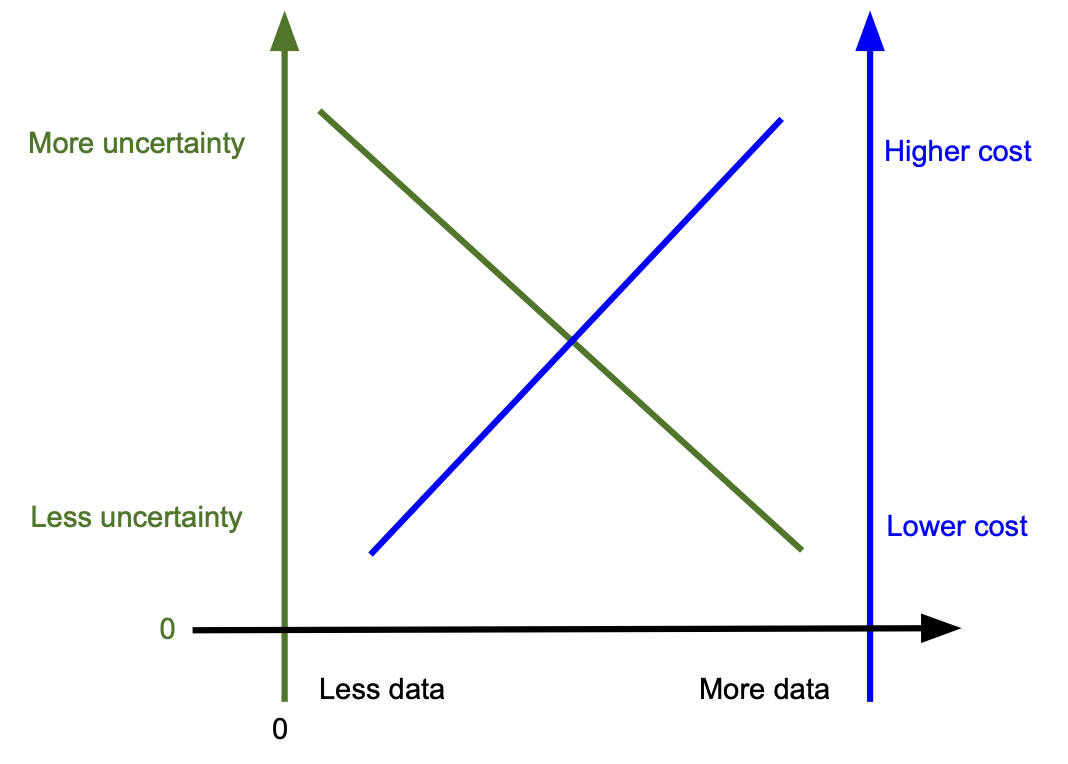
\includegraphics[width=0.8\textwidth]{images/cost_and_uncertainty_for_data_collection}
        \caption{Collecting more data costs money and time and decreases uncertainty.  See the Dilemma of Data Quantity~(\ref{table:dilemma-personal-gather-data-lots-vs-little}). This plot is wrong for multiple reasons. Cost, whether temporal or financial, does not increase linearly with data quantity. Similarly, uncertainty is not linear with data quantity. Even quantifying uncertainty is challenging. }
        \label{fig:data_collection_cost_uncertainty}
\end{figure}



% explanation of context for dilemma
% How does this relate directly to bureaucracy as defined as shared resource management policymaking?
Decision-making is foundational to bureaucracy, so gathering data to inform decisions is crucial. There's typically insufficient time and resources available for this work, which results in imperfect decisions. 

The \hyperref[table:dilemma-personal-gather-data-lots-vs-little]{Dilemma of Data Quantity} 
\iftoggle{printedonpaper}{ (\ref{table:dilemma-personal-gather-data-lots-vs-little}) }{}%
is more nuanced than merely finding 
\href{https://en.wikipedia.org/wiki/Goldilocks_principle}{just the right amount} of data.
\index{Wikipedia!Goldilocks principle@\href{https://en.wikipedia.org/wiki/Goldilocks_principle}{Goldilocks principle}}\iftoggle{WPinmargin}{\marginpar{$>$Wikipedia: Goldilocks principle}}{}
The skill is knowing which data is most relevant to the decision and having relationships with data owners to ease the cost of gathering data.

% How does this effect your relationships with other bureaucrats?
The logistics of gathering data can be measured, but there are other subjective aspects to account for as well. Making a decision has an emotional toll on the decider due to the risk of failure. Also, decisions are made in a social context, with decision-makers accounting for the ramifications on people they have relationships with. 
%The \hyperref[table:dilemma-personal-gather-data-lots-vs-little]{Dilemma of Data Quantity}

% Are the incentive structures aligned to support one direction or the other?
While gathering less data means less cost for the bureaucrat facing a decision, you might imagine some accountability for bad decisions due to inadequate data. To shield individual bureaucrats from reputation-harming liability, a decision may require an approval chain. That review process diffuses responsibility for decisions.


The \hyperref[table:dilemma-personal-gather-data-lots-vs-little]{Dilemma of Data Quantity} 
 is distinct from the \hyperref[table:dilemma-personal-planning-vs-iterate]{Dilemma of Planning}\iftoggle{printedonpaper}{ (\ref{table:dilemma-personal-planning-vs-iterate}).}{.} 
 It 
is possible to do a lot of planning with only a little information gathered, and it is feasible to have lots of data and do no planning. 

\begin{center}
\begin{table}[H] % ht
\begin{tabular}{ | m{\dilemmatablewidth}| m{\dilemmatablewidth} | } 
  \hline
  \textbf{Extensive planning upfront (proactive).} & 
  \textbf{Iterative improvement of plans (reactive).} \\ 
  \hline
  \textit{Description}: Lots of time spent brainstorming potential scenarios and contingency options before taking action. & 
  \textit{Description}: Start taking action and use feedback to shape next actions. \\ 
  \hline
  \textit{Cons}: ``No plan survives contact with the enemy.'' {\small -\href{https://en.wikipedia.org/wiki/Helmuth_von_Moltke_the_Elder}{von Moltke}
  \index{Wikipedia!Moltke@\href{https://en.wikipedia.org/wiki/Helmuth_von_Moltke_the_Elder}{Moltke, Helmuth von}}
  } & 
  % initially the citation to Wiki page was a footnote, but footnote doesn't work inside a table
  % second approach was to use \footnotemark and \footnotetext[1]{link} as per https://tex.stackexchange.com/a/109470/235813 but the footnote ended up on the next page with the wrong index
  \textit{Cons}: Less prepared. \\  
  \hline
\end{tabular}
\caption{
\textit{Dilemma of Planning.}
\index{dilemma!of planning}
How much time to invest in different types of planning.
}
\label{table:dilemma-personal-planning-vs-iterate}
%GV     "dilemma-personal-planning-vs-iterate" [label="how much planning", shape="box"];
%GV     "dilemma-personal-planning-vs-iterate" -> "plan";
%GV     "dilemma-personal-planning-vs-iterate" -> "iterate";
\end{table}
\end{center}

% explanation of context for dilemma
Managing a shared resource requires more than just on-the-spot decision-making. Thinking ahead to potential scenarios that effect the shared resource is the responsibility of the bureaucrat. 

% How does this relate directly to bureaucracy as defined as shared resource management policymaking?
The \hyperref[table:dilemma-personal-planning-vs-iterate]{Dilemma of Planning} 
\iftoggle{printedonpaper}{ (\ref{table:dilemma-personal-planning-vs-iterate}) }{}%
identifies a widely applicable challenge for bureaucrats throughout an organization (top to bottom, and on every team). Regardless of whether you're planning your next day or the next few years, there will be unforeseen challenges. Do those interruptions invalidate the effort of planning?

% How does this effect your relationships with other bureaucrats?
The \hyperref[table:dilemma-personal-planning-vs-iterate]{Dilemma of Planning} induces different responses for each bureaucrat, so you will likely encounter both someone who you think plans too much and someone who doesn't plan enough. Being exclusively reactionary can be demoralizing, as can seeing your plans become moot.

% Are the incentive structures aligned to support one direction or the other?



Making a decision imposes a bound on how much time is available for both gathering data and planning. More time gathering data is less time planning. Similarly, the number of people available for data gathering and planning is bounded, and tasking people is a zero sum choice.

\begin{figure}[H] % ht
    \centering
    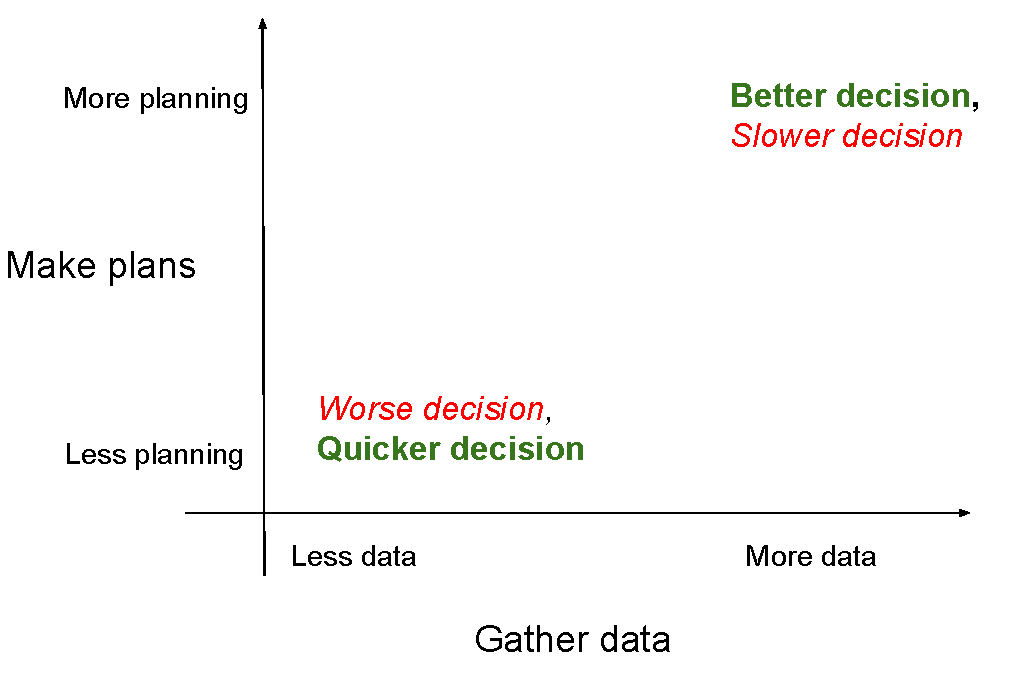
\includegraphics[width=0.8\textwidth]{images/planning_and_data_gathering.pdf}
    \caption{The trade-off of Planning (Dilemma~\ref{table:dilemma-personal-planning-vs-iterate}) and data gathering (Dilemma~\ref{table:dilemma-personal-gather-data-lots-vs-little}).}
    \label{fig:pareto_frontier}
\end{figure}

%In practice, gathering data and planning rarely stop -- they evolve.



When planning (Dilemma~\ref{table:dilemma-personal-planning-vs-iterate}), aspects to consider include
%\begin{itemize}
%    \item 
the amount of risk seeking or risk tolerance (Dilemma~\ref{table:dilemma-personal-risk-high-vs-low})
and
%    \item 
the intended scope of effect  (Dilemma~\ref{table:dilemma-personal-scope-broad-vs-narrow}).
%\end{itemize}

\begin{center}
\begin{table}[H] % ht
\begin{tabular}{ | m{\dilemmatablewidth}| m{\dilemmatablewidth} | } 
  \hline
  \textbf{Take on big risks and big rewards.} & 
  \textbf{Take on small risks and small rewards.} \\ 
  \hline
  \textit{Description}: High risk tolerance. &
  \textit{Description}: Low risk tolerance. \\
  \hline
  \textit{Pros}: Potential for failure and harm is significant. &
  \textit{Pros}: If any one investment fails, you can continue other efforts. \\
  \hline
  \textit{Cons}: Costly investment, longer feedback cycle. & 
  \textit{Cons}: Incremental can be slower. \\
  \hline
\end{tabular}
\caption{
\textit{Dilemma of \href{https://en.wikipedia.org/wiki/Risk_assessment}{Risk tolerance}.
\index{Wikipedia!risk tolerance@\string\href{https://en.wikipedia.org/wiki/Risk_assessment}{risk tolerance}}
} 
\index{dilemma!of risk tolerance@of \string\href{https://en.wikipedia.org/wiki/Risk_assessment}{risk tolerance}}
%{\tiny Tag: Personal choice.}
}
\label{table:dilemma-personal-risk-high-vs-low}
%GV     "dilemma-personal-risk-high-vs-low" [label="big risk or small risk", shape="box"];
%GV     "dilemma-personal-risk-high-vs-low" -> "risk";
\end{table}
\end{center}

% explanation of context for dilemma
Taking big leaps can be exciting. But you might be leaping to failure. Small leaps are less risky, supporting an evolutionary path to discovery. 

% How does this relate directly to bureaucracy as defined as shared resource management policymaking?
The \hyperref[table:dilemma-personal-risk-high-vs-low]{Dilemma of Risk Tolerance} 
\iftoggle{printedonpaper}{ (\ref{table:dilemma-personal-risk-high-vs-low}) }{}%
arises in bureaucracy because the environment around the shared resource being managed isn't static. Change requires policies and processes to change. Whether the change is small or large is dependent on the risk tolerance of individual bureaucrats involved in the decision. 

% How does this effect your relationships with other bureaucrats?
The risk tolerance of individuals is shaped by their experience. What you see as conventional and routine another bureaucrat would regard as untested. 

%The \hyperref[table:dilemma-personal-risk-high-vs-low]{Dilemma of Risk Tolerance}
% Are the incentive structures aligned to support one direction or the other?
The bias for bureaucrats is towards smaller risks. That way if failure does occur the bureaucrat incurs less harm to their reputation. As a consequence, significant 
\hyperref[sec:innovation]{innovation} is difficult in bureaucratic organizations. 


\begin{center}
\begin{table}[H]
\begin{tabular}{ | m{\dilemmatablewidth}| m{\dilemmatablewidth} | } 
  \hline
  \textbf{Involve people who disagree.} & 
  \textbf{Ignore people who disagree.} \\ 
  \hline
  \textit{Pros}: Get constructive feedback; account for factors you didn't consider; build a robust solution. & 
  \textit{Pros}: Save time by not interacting. \\  
  \hline
  \textit{Cons}: Results in a compromise or partial solution that minimizes aggregate unhappiness. & 
  \textit{Cons}: Miss a vital aspect you didn't consider. \\  
  \hline
\end{tabular}
\caption{\textit{Dilemma of Disagreement.}
\index{dilemma!of disagreement}
Engagement with opposition to process or change.
}
\label{table:dilemma-personal-opposition-involve-ignore}
%GV     "dilemma-personal-opposition-involve-ignore" [label="involve opposition or ignore", shape="box"];
%GV     "dilemma-personal-opposition-involve-ignore" -> "disagree";
\end{table}
\end{center}

%  explanation of context for dilemma


% How does this relate directly to bureaucracy as defined as shared resource management policymaking?
Bureaucracy is the subjective decision-making associated with management of shared resources, so the existence of people who disagree is not surprising. The choice you face is whether to engage with people who think you're wrong. 

% How does this effect your relationships with other bureaucrats?
The \hyperref[table:dilemma-personal-opposition-involve-ignore]{Dilemma of Disagreement} is sensitive to how social you are and how well you can negotiate. If you can hear criticism of your idea and not take it personally, you are more capable of getting constructive feedback. Having relationships where that level of honesty is available is a long-term investment.

%
% Are the incentive structures aligned to support one direction or the other?
The default behavior for bureaucrats facing the \hyperref[table:dilemma-personal-opposition-involve-ignore]{Dilemma of Disagreement} is to avoid negative input. What you might consider innovation another person might see as wasteful. To avoid that risk, don't share what you're working on.

\begin{center}
\begin{table}[H] % ht
\begin{tabular}{ | m{\dilemmatablewidth}| m{\dilemmatablewidth} | } 
  \hline
  \textbf{Broad scope of effect.} &
  \textbf{Narrow scope of effect.} \\
  \hline
  \textit{Description}: The consequence of the work has many stakeholders. &
  \textit{Description}: Small number of stakeholders. \\  
  \hline
  \textit{Pros}: Help more people. &
  \textit{Pros}: Niche effect means fewer dependencies on other people. \\
  \hline
  \textit{Cons}: Harder to get everyone in agreement. & 
  \textit{Cons}: Less visibility to the rest of the organization. \\
  \hline
\end{tabular}
\caption{
\textit{Dilemma of Scope of Effect.}
\index{dilemma!of scope of effect}
Scope of the effect of your work. 
%{\tiny Tag: Personal choice}
}
\label{table:dilemma-personal-scope-broad-vs-narrow}
%GV     "dilemma-scope-broad-vs-narrow" [label="scope of effect broad vs narrow", shape="box"];
%GV     "dilemma-scope-broad-vs-narrow" -> "scope";
\end{table}
\end{center}

% explanation of context for dilemma
Framed as ``Should you work on something consequential?" the na\"ive answer is to say yes. However, to make effective change involves coordinating more stakeholders than you may be comfortable with. Experienced bureaucrats are more likely to carve off a small portion of a big challenge.

% How does this relate directly to bureaucracy as defined as shared resource management policymaking?
You may have some freedom to choose what you work on, in which case the \hyperref[table:dilemma-personal-scope-broad-vs-narrow]{Dilemma of Scope of Effect} is in play. Mentorship from more experienced bureaucrats can help you decide what scope of task is big enough to be meaningful but not too big as to be intractable.

% How does this effect your relationships with other bureaucrats?
%The \hyperref[table:dilemma-personal-scope-broad-vs-narrow]{Dilemma of Scope of Effect}
% Are the incentive structures aligned to support one direction or the other?


\ \\

Once \hyperref[table:dilemma-personal-gather-data-lots-vs-little]{data is gathered} (Dilemma~\ref{table:dilemma-personal-gather-data-lots-vs-little}) and a \hyperref[table:dilemma-personal-planning-vs-iterate]{plan is made} (Dilemma~\ref{table:dilemma-personal-planning-vs-iterate}), the result is disseminated. The choices of how to disseminate are the \hyperref[table:dilemma-personal-consistency-gradual-stepwise]{Dilemma of Consistency over time} (\ref{table:dilemma-personal-consistency-gradual-stepwise}) and the \hyperref[table:dilemma-personal-disseminate-one-by-one]{Dilemma of Disseminating information} (\ref{table:dilemma-personal-disseminate-one-by-one}).

\begin{center}
\begin{table}[H] % ht
\begin{tabular}{ | m{\dilemmatablewidth}| m{\dilemmatablewidth} | } 
  \hline
  \textbf{Guidance updated often; incremental change.} & 
  \textbf{Consistent application of policy over time. Rules persist; then sudden drastic change.} \\ 
  \hline
  \textit{Pros}: Adapt policy to new information and changing conditions. &
  \textit{Pros}: Stability is easier to predict between regime changes.  \\
  \hline
  \textit{Cons}: More work needed for revisions. Accused of lacking stability. & 
  \textit{Cons}: Doesn't adapt as conditions change. Accused of being inflexible to evolving conditions. \\
  \hline
\end{tabular}
\caption{
\textit{Dilemma of Consistency over time.} 
\index{dilemma!of consistency over time}
Stability of rules; how change is enacted. Can also be characterized as when to tell other people: sooner (decreases surprise) or later (when firmer information is available).
See the description of \hyperref[sec:static-dynamic-processes]{static versus dynamic processes}\iftoggle{haspagenumbers}{ on page~\pageref{sec:static-dynamic-processes}.}{.}
%\ifpageref
%on page~\pageref{sec:static-dynamic-processes}
%\fi
%\iftoggle{pageref}{%
%on page~\pageref{sec:static-dynamic-processes}
%}
%\iftoggle{sectionref}{%
%in section~\ref{sec:static-dynamic-processes} 
%}
%{\tiny Tag: Organization's culture. Tag: Personal choice.}
}
\label{table:dilemma-personal-consistency-gradual-stepwise}
%GV     "dilemma-personal-consistency-gradual-stepwise" [label="incremental or step-wise change", shape="box"];
%GV     "dilemma-personal-consistency-gradual-stepwise" -> "consistency";
\end{table}
\end{center}

Deployment of products in industry and deployment of policies in a bureaucracy face similar dilemmas. The \href{https://en.wikipedia.org/wiki/Diffusion_of_innovations}{Diffusion of Innovation} 
\index{Wikipedia!diffusion of innovation@\href{https://en.wikipedia.org/wiki/Diffusion_of_innovations}{diffusion of innovation}}
describes how innovation is adopted by people with different amounts of risk tolerance.

% How does this relate directly to bureaucracy as defined as shared resource management policymaking?
Bureaucracy exists to manage access to shared resources. Management occurs by policies and processes. The community accessing the shared resource changes over time, so the policies and processes evolve to reflect that change. The \hyperref[table:dilemma-personal-consistency-gradual-stepwise]{Dilemma of Consistency over time} is about the degree of incrementalism of the change.

% How does this effect your relationships with other bureaucrats?
Bureaucrats responsible for carrying out policies and processes disagree on the question of stability. This disagreement generates friction for other processes reliant on those relations within an organization.
The \hyperref[table:dilemma-personal-consistency-gradual-stepwise]{Dilemma of Consistency over time} is also disruptive to the subjects of bureaucracy. 

% Are the incentive structures aligned to support one direction or the other?
Bureaucrats are incentivized to avoid change, so the bias in this dilemma is towards consistency and stability even if that means not adapting to current local circumstances. 

\begin{center}
\begin{table}[H] % ht
\begin{tabular}{ | m{\dilemmatablewidth}| m{\dilemmatablewidth} | } 
  \hline
  \textbf{Tell people one-by-one.} & 
  \textbf{Tell everyone at once.} \\ 
  \hline
  \textit{Pros}: One-on-one allows a freer response from the audience. &
  \textit{Pros}: Saves time for the speaker. \\
  \hline
  \textit{Cons}: Order matters for relationships. & 
  \textit{Cons}: Overwhelming feedback all at once. Some people don't feel heard. \\  
  \hline
\end{tabular}
\caption{
\textit{Dilemma of Disseminating information.}
\index{dilemma!of disseminating information}
%{\tiny Tag: Personal choice.}
}
\label{table:dilemma-personal-disseminate-one-by-one}
%GV     "dilemma-personal-disseminate-one-by-one" [label="notify one-by-one ar at once", shape="box"];
%GV     "dilemma-personal-disseminate-one-by-one" -> "";
\end{table}
\end{center}

Once a decision has been made, the decision is executed or enforced. \hyperref[table:dilemma-personal-number-of-rules]{How many rules are there} (Dilemma~\ref{table:dilemma-personal-number-of-rules}) and
\hyperref[table:dilemma-personal-rule-strictness-lax]{how strictly are the rules enforced} (Dilemma~\ref{table:dilemma-personal-rule-strictness-lax})?

% How does this relate directly to bureaucracy as defined as shared resource management policymaking?
Bureaucracy involves coordination to facilitate distributed knowledge and distributed decision-making. Each bureaucrat has finite time and attention. When communication channels are instantaneous (e.g., phone, email, video), there is often more information to be consumed.
The \hyperref[table:dilemma-personal-disseminate-one-by-one]{Dilemma of Disseminating information} is a question of whether to save time by telling all stakeholders at one time or demonstrate the importance of a relationship by talking one-on-one. 

% How does this effect your relationships with other bureaucrats?

One aspect of the \hyperref[table:dilemma-personal-disseminate-one-by-one]{Dilemma of Disseminating information} can be addressed using personalized emails. Rather than send an email notice to ten people, automating the process of sending ten separate emails can make it appear to each recipient that the conversation is one-on-one.  That doesn't resolve the challenge of getting all feedback at once.

% Are the incentive structures aligned to support one direction or the other?
Whether to talk informally before a formal interaction (\href{https://en.wikipedia.org/wiki/Nemawashi}{nemawashi}) 
\index{Wikipedia!nemawashi@\href{https://en.wikipedia.org/wiki/Nemawashi}{nemawashi}}\iftoggle{WPinmargin}{\marginpar{$>$Wikipedia: Nemawashi}}{}
or not depends on how much time to allocate to sharing the information. 

\begin{center}
\begin{table}[H] % ht
\begin{tabular}{ | m{\dilemmatablewidth}| m{\dilemmatablewidth} | } 
  \hline
  \textbf{Enforce rules strictly.} & 
  \textbf{Lax rule enforcement.} \\ 
  \hline
  \textit{Pros}: Predictable. &
  \textit{Pros}: Bureaucrats feel empowered. Tolerance for changing conditions or exceptional cases. \\
  \hline
  \textit{Cons}: Insensitive to nuance. & 
  \textit{Cons}: Enforcement is subjective and unpredictable.  \\  
  \hline
\end{tabular}
\caption{
\textit{Dilemma of Strictness of rules.}
\index{dilemma!of strictness of rules}
%{\tiny Tag: Organization's culture.}
}
\label{table:dilemma-personal-rule-strictness-lax}
%GV     "dilemma-personal-rule-strictness-lax" [label="enforce rules strict or lax", shape="box"];
%GV     "dilemma-personal-rule-strictness-lax" -> "rules";
\end{table}
\end{center}

% How does this relate directly to bureaucracy as defined as shared resource management policymaking?
Bureaucracy is the subjective decision-making associated with shared resources. Interpretation of rules and enforcement of rules is not objective. Bureaucrats are empowered to make trade-offs specific to the circumstances being considered.

% explanation of context for dilemma

The 
\hyperref[table:dilemma-personal-rule-strictness-lax]{Dilemma of Strictness of rules} 
is about how the bureaucrat enforcing policies decides to act, whereas the
\hyperref[table:dilemma-subject-consistency-per-situation]{Dilemma of Consistency} 
(whether to seek exceptions) and
\hyperref[table:dilemma-subject-flexibility]{Dilemma of Flexible Rules}
are from the subject's view. While the objective question is similar, the rationalization for behavior depends on which role is being considered.

Bureaucrats and subjects of bureaucracy both complain regardless of where on the spectrum each instance of the \hyperref[table:dilemma-personal-rule-strictness-lax]{Dilemma of Strictness of rules} occurs. 

% How does this effect your relationships with other bureaucrats?
Different bureaucrats will evaluate which rules apply in each circumstance slightly differently (which provides another opportunity to apply your Process Empathy). Barring consensus, the organization's hierarchy is used to having one person decide what the relevant interpretation is.

% Are the incentive structures aligned to support one direction or the other?
The default behavior is strict enforcement since that is a defensible story for the responsible bureaucrat. Exceptions based on personal relationships do not appear fair to outsiders.


\begin{center}
\begin{table}[H] % ht
\begin{tabular}{ | m{\dilemmatablewidth}| m{\dilemmatablewidth} | } 
  \hline
  \textbf{Control via rules.} & 
  \textbf{Freedom, autonomy, agility.} \\ 
  \hline
  \textit{Description}: High number of rules to cover various situations. & 
  \textit{Description}: Low number of rules to enable flexibility. \\ 
  \hline
  \textit{Cons}: The more rules that exist, the more likely it is that someone will find a way to exploit them to their advantage. & 
  \textit{Cons}: The fewer rules that exist, the more likely it is that someone will try to get away with something bad. \\  
  \hline
\end{tabular}
\caption{
\textit{Dilemma of Number of rules.}
\index{dilemma!of number of rules}
%{\tiny Tag: Organization's culture}
}
\label{table:dilemma-personal-number-of-rules}
%GV     "dilemma-personal-number-of-rules" [label="rule or freedom", shape="box"];
%GV     "dilemma-personal-number-of-rules" -> "rules";
\end{table}
\end{center}



%  explanation of context for dilemma
% How does this relate directly to bureaucracy as defined as shared resource management policymaking?
The \hyperref[table:dilemma-personal-number-of-rules]{Dilemma of Number of rules}
\marginpar{$>>$ \href{https://en.wikipedia.org/wiki/Goldilocks_principle}{Goldilocks balance}}%
\index{Goldilocks balance!number of rules}%
arises in bureaucratic organizations because bureaucrats have to make subjective decisions about shared resources. 

% How does this effect your relationships with other bureaucrats?
%The \hyperref[table:dilemma-personal-number-of-rules]{Dilemma of Number of rules}
% Are the incentive structures aligned to support one direction or the other?

An alternative approach to the  \hyperref[table:dilemma-personal-number-of-rules]{Dilemma of Number of rules}
is to use guidance derived from principles. A principles-based approach relies on good judgment which can be adapted to specific situations. What qualifies as ``good'' has subjective boundary conditions and requires knowledge of the situation.



\begin{center}
\begin{table}[H] % ht
\begin{tabular}{ | m{\dilemmatablewidth}| m{\dilemmatablewidth} | } 
  \hline
  \textbf{If it's not against the rules, it must be okay.} & 
  \textbf{I can only do what is allowed by the rules and nothing more.} \\ 
  \hline
  \textit{Description}: I can do anything that's not illegal. &
  \textit{Description}: Do only what is mandated by the organization. \\
  \hline
  \textit{Pros}: Autonomy, flexibility. &
  \textit{Pros}: Less risk of getting in trouble. \\
  \hline
  \textit{Cons}: What one person deems reasonable, another may not. & 
  \textit{Cons}: Constrains creative solutions. Less productive. Responding to novel situations is inhibited. \\  
  \hline
\end{tabular}
\caption{
\textit{Dilemma of Adherence to Rules} depends on an individual's risk tolerance versus aversion to risk. 
The scope of your actions is bound by mandates and legality, but the way you interpret that is subjective. 
Constraining activities to explicitly specified rules can be used as an excuse for laziness. 
\index{dilemma!of adherence to rules}
}
\label{table:dilemma-personal-rule-adherence}
%GV     "dilemma-personal-rule-adherence" [label="rules allow or conform", shape="box"];
%GV     "dilemma-personal-rule-adherence" -> "rules";
\end{table}
\end{center}

%  explanation of context for dilemma
Your understanding of your freedom versus responsibilities may be a philosophical topic, but it can manifest in bureaucratic organizations. Being a member of an organization means leveraging the resources available or acting in accordance with mandates. 
% How does this relate directly to bureaucracy as defined as shared resource management policymaking?
The \hyperref[table:dilemma-personal-rule-adherence]{Dilemma of Adherence to Rules}\footnote{See Wikipedia entry \href{https://en.wikipedia.org/wiki/Everything_which_is_not_forbidden_is_allowed}{Everything which is not forbidden is allowed}. 
\index{Wikipedia!everything which is not forbidden is allowed@\string\href{https://en.wikipedia.org/wiki/Everything_which_is_not_forbidden_is_allowed}{everything which is not forbidden is allowed}}} is used by bureaucrats to rationalize their action (or inaction). 

% How does this effect your relationships with other bureaucrats?
There are a few tactics you can use when you encounter a coworker who disagrees with your understanding of which side of the \hyperref[table:dilemma-personal-rule-adherence]{Dilemma of Adherence to Rules} your organization operates. 
Changing a coworker's attitude on this dichotomy depends on the origin of their stance. You can use appeals to authority or provide emotional reassurance.

%The \hyperref[table:dilemma-personal-rule-adherence]{Dilemma of Adherence to Rules}
% Are the incentive structures aligned to support one direction or the other?

\begin{center}
\begin{table}[H] % ht
\begin{tabular}{ | m{\dilemmatablewidth}| m{\dilemmatablewidth} | } 
  \hline
  \textbf{A decision in a process is informed by a single bit of information.} & 
  \textbf{Fault-tolerant decision-making through redundancy.} \\ 
  \hline
  \textit{Description}: A form featuring a checkbox option. & 
  \textit{Description}: Multiple independent confirmations that the data collected is correct.  \\
  \hline
  \textit{Pros}: Less overhead. & 
  \textit{Pros}: Decrease mistakes. \\
  \hline
  \textit{Cons}: Single point of failure. Might be accidentally wrong. &
  \textit{Cons}: More time needed. Extra burden of collecting and processing more data. \\  
  \hline
\end{tabular}
\caption{
\textit{Dilemma of Redundant Data for Decisions.}
\index{dilemma!of redundant data for decisions}
Having a single checkbox on a form makes data collection easier for both the subject and the bureaucrat. However, the person using the form might not see the checkbox or may accidentally fill in the checkbox. Is there any validation of the selection? The process is sensitive to this single bit of data. This applies to written forms and verbal conversations. 
}
\label{table:dilemma-personal-single-bit-decision}
%GV     "dilemma-personal-single-bit-decision" [label="single bit error", shape="box"];
%GV     "dilemma-personal-single-bit-decision" -> "redundancy";
\end{table}
\end{center}

%  explanation of context for dilemma
The \hyperref[table:dilemma-personal-single-bit-decision]{Dilemma of Redundant Data for Decisions} is about the redundancy of data used for coordination. Collecting as little data as needed streamlines interactions between subjects and bureaucrats. Bureaucratic management of shared resources depends on decision-making, and decisions require information. That information should be correct, but how much investment should be made to ensure correctness?

The \hyperref[table:dilemma-personal-single-bit-decision]{Dilemma of Redundant Data for Decisions} is distinct from the \hyperref[table:dilemma-personal-gather-data-lots-vs-little]{Dilemma of Data Quantity}, which is about how much data is needed for assessing the application of policies.

% How does this relate directly to bureaucracy as defined as shared resource management policymaking?

% How does this effect your relationships with other bureaucrats?
Most decisions are of low importance, so the correctness of information is rarely checked. Redundant information is deemed wasteful, and those habits don't necessarily change when the significance of a decision increases. The lack of feedback loops motivating correct information can harm participants.

The \hyperref[table:dilemma-personal-single-bit-decision]{Dilemma of Redundant Data for Decisions} presents a lose-lose situation: collect redundant information (which introduces more risk of conflicting information) or hope that data collected represents reality without checking. 

% Are the incentive structures aligned to support one direction or the other?

\begin{center}
\begin{table}[H] % ht
\begin{tabular}{ | m{\dilemmatablewidth}| m{\dilemmatablewidth} | } 
  \hline
  \textbf{A single bureaucrat reviews information and makes a decision.} & 
  \textbf{Catch mistakes in decision-making by using multiple reviewers.} \\ 
  \hline
  \textit{Description}: A decision process relies on a single bureaucrat. & 
  \textit{Description}: Multiple independent confirmations of a decision.  \\
  \hline
  \textit{Pros}: Less overhead. & 
  \textit{Pros}: Decrease mistakes. \\
  \hline
  \textit{Cons}: Single point of failure. Might get policy interpretation wrong. &
  \textit{Cons}: More time and staffing needed. Diffuses ownership of decisions. \\  
  \hline
\end{tabular}
\caption{
\textit{Dilemma of Redundant Reviewers.}
\index{dilemma!of redundant reviewers}
Having a single bureaucrat make a decision is quicker than checking that bureaucrat. Validating the decision slows down the process and requires more bureaucrats.
}
\label{table:dilemma-personal-redundant-reviewers}
%GV     "dilemma-personal-redundant-reviewers" [label="redundant reviewers", shape="box"];
%GV     "dilemma-personal-redundant-reviewers" -> "redundancy";
\end{table}
\end{center}

% TODO: Explanation of context for dilemma
The \hyperref[table:dilemma-personal-redundant-reviewers]{Dilemma of Redundant Reviewers} extends the same concept as the \hyperref[table:dilemma-personal-single-bit-decision]{Dilemma of Redundant Data for Decisions} to humans making decisions based on the provided data. Each bureaucrat is fallible, so checking a decision for faults is a reasonable investment if the decision is significant. The challenge in this dilemma is evaluating what qualifies as worth reviewing.

% How does this relate directly to bureaucracy as defined as shared resource management policymaking?
Bureaucracy is defined as the system of distributed decision-making about shared resources, and the \hyperref[table:dilemma-personal-redundant-reviewers]{Dilemma of Redundant Reviewers} is one aspect of what is meant by distributed.

%The \hyperref[table:]{Dilemma of }
% How does this effect your relationships with other bureaucrats?
The \hyperref[table:dilemma-personal-redundant-reviewers]{Dilemma of Redundant Reviewers} presents another lose-lose choice: trusting a single bureaucrat, or diffusing responsibility among many. In the case of a single bureaucrat as the decider, other members are implicitly trusting the validity of decisions made. In the case of multiple reviewers, there is a reliance on personal relationships (``Do I trust the other participants to do their job?'') and professional expectations (``That person must know what they're doing.'')

%The \hyperref[table:]{Dilemma of }
% Are the incentive structures aligned to support one direction or the other?
The \hyperref[table:dilemma-personal-redundant-reviewers]{Dilemma of Redundant Reviewers} defaults to multiple participants because diffused responsibility is preferable for each participant. Only when a decision is trivial or there is insufficient staffing will a single bureaucrat suffice.

\begin{center}
\begin{table}[H] % ht
\begin{tabular}{ | m{\dilemmatablewidth}| m{\dilemmatablewidth} | } 
  \hline
  \textbf{Quickly complete tasks or deploy new policies or create new products.} & 
  \textbf{Methodically complete tasks (or well-founded policies, quality products).} \\ 
  \hline
  \textit{Description}: Enact a solution quickly to address urgent needs. &
  \textit{Description}: Methodical well-planned design and execution yield robust solutions/products/policies. \\
  \hline
  \textit{Pros}: Rapid solution. &
  \textit{Pros}: More like to get the solution right. \\
  \hline
  \textit{Cons}: Risk of a quick task is that the result is ineffective, inefficient, or wrong. &
  \textit{Cons}: \href{https://en.wikipedia.org/wiki/Opportunity_cost}{opportunity cost}. 
  \index{Wikipedia!opportunity cost@\href{https://en.wikipedia.org/wiki/Opportunity_cost}{opportunity cost}}
  \\  
  \hline
\end{tabular}
\caption{
\textit{Dilemma of Speed and Accuracy.}
\index{dilemma!of speed and accuracy}
Speed versus accuracy of task completion.
}
\label{table:dilemma-personal-quick-methodical}
%GV     "dilemma-personal-quick-methodical" [label="quick or methodical", shape="box"];
%GV     "dilemma-personal-quick-methodical" -> "speed";
\end{table}
\end{center}

If you try to resolve the \hyperref[table:dilemma-personal-quick-methodical]{Dilemma of Speed and Accuracy} by both getting a solution deployed quickly and then iterating towards a robust outcome, you may appear unpredictable or unstable; see Dilemma~\ref{table:dilemma-personal-planning-vs-iterate}. This is an example of cascading dilemmas. The interplay of a creative resolution to one dilemma can affect the solution space for other dilemmas. 

%  explanation of context for dilemma
% How does this relate directly to bureaucracy as defined as shared resource management policymaking?
%The \hyperref[table:dilemma-personal-quick-methodical]{Dilemma of Speed and Accuracy}
% How does this effect your relationships with other bureaucrats?
Regardless of where on this spectrum you are with the \hyperref[table:dilemma-personal-quick-methodical]{Dilemma of Speed and Accuracy}, someone that you depend on in the bureaucracy will take the opposite stance. This becomes a source of friction regarding how long tasks should take. 

% Are the incentive structures aligned to support one direction or the other?
The bias for this dilemma is that most bureaucrats want to be perceived as methodical and careful. Quick judgment is seen as risky. 


\begin{center}
\begin{table}[H] % ht
\begin{tabular}{ | m{\dilemmatablewidth}| m{\dilemmatablewidth} | } 
  \hline
  \textbf{Push people to work hard.} & 
  \textbf{Create a comfortable work environment.} \\ 
  \hline
  \textit{Cons}: Burn out and leave. & 
  \textit{Cons}: Lower instantaneous productivity. \\  
  \hline
\end{tabular}
\caption{
\textit{Dilemma of Urgency.}
\index{dilemma!of urgency}
}
\label{table:dilemma-personal-manager-rate-of-work}
%GV     "dilemma-personal-manager-rate-of-work" [label="work hard or sustainably", shape="trapezium"];
%GV     "dilemma-personal-manager-rate-of-work" -> "level-of-effort";
%GV     "dilemma-personal-manager-rate-of-work" -> "dilemma-personal-work-extra-or-work-as-expected" [dir=none];
\end{table}
\end{center}

% How does this relate directly to bureaucracy as defined as shared resource management policymaking?
There is usually a large range of productivity possible for a bureaucrat. Management has input on what is expected from 
 a bureaucrat. The 
\hyperref[table:dilemma-personal-manager-rate-of-work]{Dilemma of Urgency} reflects the trade-off of how much to push employees of an organization. The \hyperref[table:dilemma-personal-manager-rate-of-work]{Dilemma of Urgency} is the manager's perspective, whereas the
\hyperref[table:dilemma-personal-work-extra-or-work-as-expected]{Dilemma of Working Extra Hard}
is the view of the bureaucrat. 

% How does this effect your relationships with other bureaucrats?
%The \hyperref[table:dilemma-personal-manager-rate-of-work]{Dilemma of Urgency}

% Are the incentive structures aligned to support one direction or the other?
Because of weak feedback loops in bureaucratic organizations, bureaucrats default to a relaxed work environment. Examples of exceptions to this include seasonal variations like tax collection time for the \href{https://en.wikipedia.org/wiki/Internal_Revenue_Service}{IRS} 
\index{Wikipedia!Internal Revenue Service@\href{https://en.wikipedia.org/wiki/Internal_Revenue_Service}{Internal Revenue Service}}%
\index{exemplar!Internal Revenue Service@\href{https://en.wikipedia.org/wiki/Internal_Revenue_Service}{Internal Revenue Service (IRS)}}%
and demand spikes like a natural disaster for \href{https://en.wikipedia.org/wiki/Federal_Emergency_Management_Agency}{FEMA}. 
\index{Wikipedia!Federal Emergency Management Agency@\href{https://en.wikipedia.org/wiki/Federal_Emergency_Management_Agency}{Federal Emergency Management Agency}}
\index{exemplar!Federal Emergency Management Agency@\href{https://en.wikipedia.org/wiki/Federal_Emergency_Management_Agency}{Federal Emergency Management Agency (FEMA)}}

% https://bennorthrop.com/Essays/2022/code-ownership-stewardship-or-free-for-all.php
\begin{center}
\begin{table}[H] % ht
\begin{tabular}{ | m{\dilemmatablewidth}| m{\dilemmatablewidth} | } 
  \hline
  \textbf{Talk more to convey more information.} & 
  \textbf{Listen more to learn more information.} \\ 
  \hline
  \textit{Cons}: Less time available for listening. & 
  \textit{Cons}: Less time to convey what you know. \\  
  \hline
\end{tabular}
\caption{
\textit{Dilemma of Talking.}
\index{dilemma!of talking}
In conversations or meetings there is a (subjective) balance for participants.
}
\label{table:dilemma-personal-talk-or-listen}
%GV     "dilemma-personal-talk-or-listen" [label="talk or listen", shape="box"];
%GV     "dilemma-personal-talk-or-listen" -> "speak";
\end{table}
\end{center}

% How does this relate directly to bureaucracy as defined as shared resource management policymaking?
The \hyperref[table:dilemma-personal-talk-or-listen]{Dilemma of Talking}%
captures the zero-sum information constraint that most bureaucrats can't concurrently talk and listen. 

% How does this effect your relationships with other bureaucrats?
The \hyperref[table:dilemma-personal-talk-or-listen]{Dilemma of Talking} depends on the personality of each bureaucrat involved in the coordination of distributed knowledge and distributed decision-making. Some are patient listeners, while others feel uncomfortable with silence.

% Are the incentive structures aligned to support one direction or the other?
Talking constructively about work takes effort, so the default here is to not communicate. 


\begin{center}
\begin{table}[H] % ht
\begin{tabular}{ | m{\dilemmatablewidth}| m{\dilemmatablewidth} | } 
  \hline
  \textbf{Seek out experienced collaborators.} & 
  \textbf{Work with less experienced people.} \\ 
  \hline
  \textit{Pros}: Quicker to get something done. &
  \textit{Pros}: Less set in their ways and open to more novelty. \\  
  \hline
  \textit{Cons}: Experienced people who are good are probably busy. &
  \textit{Cons}: Slower progress; more education needed. \\  
  \hline
\end{tabular}
\caption{
\textit{Dilemma of Experienced Collaborators.}
\index{dilemma!of experienced collaborators}
People with experience are useful but less accessible.
}
\label{table:dilemma-personal-experienced-collaborators}
%GV     "dilemma-personal-experienced-collaborators" [label="experienced collaborators or not", shape="box"];
%GV     "dilemma-personal-experienced-collaborators" -> "";
\end{table}
\end{center}


% How does this relate directly to bureaucracy as defined as shared resource management policymaking?
Distributed knowledge in a bureaucracy relies on collaboration among bureaucrats. 
The \hyperref[table:dilemma-personal-experienced-collaborators]{Dilemma of Experienced Collaborators} is 
\iftoggle{printedonpaper}{ (\ref{table:dilemma-personal-experienced-collaborators})}{}about the options of who to collaborate with. 

% How does this effect your relationships with other bureaucrats?

% Are the incentive structures aligned to support one direction or the other?
The bias for the \hyperref[table:dilemma-personal-experienced-collaborators]{Dilemma of Experienced Collaborators} depends on the promotion structure of your organization and the composition of the workforce. If training new members of the team is rewarded, then you might choose to work with less experienced bureaucrats. If the entire team is experienced, then this Dilemma doesn't apply.

\begin{center}
\begin{table}[H] % ht
\begin{tabular}{ | m{\dilemmatablewidth}| m{\dilemmatablewidth} | } 
  \hline
  \textbf{Say yes to new opportunities.} & 
  \textbf{Say no to new opportunities.} \\ 
  \hline
  \textit{Pros}: Positive attitude, collaborative. &
  \textit{Pros}: Able to prioritize and focus. \\
  \hline
  \textit{Cons}: Fail to complete tasks. &
  \textit{Cons}: Not a team player. \\  
  \hline
\end{tabular}
\caption{
\textit{Dilemma of opportunities.}
\index{dilemma!of opportunities}
Acceptance or rejection of more work can be explicit or implicit. Bureaucrats respond to this challenge by sending mixed signals: expressing interest but not following up with action.
}
\label{table:dilemma-new-opportunties-yes-no}
%GV     "dilemma-new-opportunties-yes-no" [label="new opportunities yes or no", shape="box"];
%GV     "dilemma-new-opportunties-yes-no" -> "";
\end{table}
\end{center}

% How does this relate directly to bureaucracy as defined as shared resource management policymaking?
The \hyperref[table:dilemma-new-opportunties-yes-no]{Dilemma of Opportunities} 
\iftoggle{printedonpaper}{ (\ref{table:dilemma-new-opportunties-yes-no}) }{}%
depends as much on the workload as on your personality. 

% How does this effect your relationships with other bureaucrats?
Finding ways to avoid doing work while helping the person providing the opportunity is the central skill for the \hyperref[table:dilemma-new-opportunties-yes-no]{Dilemma of Opportunities}. This may mean referring the opportunity to another coworker or expressing support but not investing effort. 

% Are the incentive structures aligned to support one direction or the other?


\begin{center}
\begin{table}[H] % ht
\begin{tabular}{ | m{\dilemmatablewidth}| m{\dilemmatablewidth} | } 
  \hline
  \textbf{Share less data.} &
  \textbf{Share more data.} \\
%  \hline
%  \textit{Description}:  &
%  \textit{Description}:  \\  
  \hline
  \textit{Pros}: Restricting data access saves money and time for the data owner.&
  \textit{Pros}: Sharing data improves transparency and accountability. \\
  \hline
  \textit{Cons}: People other than the data owner are unable to extract value from data. & 
  \textit{Cons}: Sharing data uses resources (people, money, time). \\
  \hline
\end{tabular}
\caption{
\textit{Dilemma of Sharing Data.}
\index{dilemma!of sharing data}
How much data to share. A potential solution is to make data discoverable. Advertise the availability of data without providing data. Then negotiation is feasible for people interested in the data.
%{\tiny Tag: Personal choice.}
}
\label{table:dilemma-data-share-vs-hide}
%GV     "dilemma-data-share-vs-hide" [label="share data less or more", shape="box"];
%GV     "dilemma-data-share-vs-hide" -> "share";
%GV     "dilemma-data-share-vs-hide" -> "data";
\end{table}
\end{center}

In the \hyperref[table:dilemma-data-share-vs-hide]{Dilemma of Sharing Data} 
\iftoggle{printedonpaper}{ (\ref{table:dilemma-data-share-vs-hide}) }{}%
there are many of aspects of data that can be 
shared to improve discoverability: who to contact about access, what the data sources are, how often data is collected, how long data is stored, and how much data exists.

% How does this relate directly to bureaucracy as defined as shared resource management policymaking?
Distributed knowledge and distributed decision-making both rely on having data. Without data, the policies and processes of bureaucracy are less effective. 

% How does this effect your relationships with other bureaucrats?
Sharing data is typically perceived as helpful. 
The \hyperref[table:dilemma-data-share-vs-hide]{Dilemma of Sharing Data} 
\iftoggle{printedonpaper}{ (\ref{table:dilemma-data-share-vs-hide}) }{}%
points out that helpfulness has a cost. 

% Are the incentive structures aligned to support one direction or the other?
Because sharing data consumes resources, the bias is to not provide data. That applies to sharing with other bureaucrats within the organization as well as subjects of the bureaucracy. 


\begin{center}
\begin{table}[H] % ht
\begin{tabular}{ | m{\dilemmatablewidth}| m{\dilemmatablewidth} | } 
  \hline
  \textbf{Compete for resources.} &
  \textbf{Cooperate for productivity.} \\
  \hline
  \textit{Description}: individuals compete for attention and promotion; teams compete for money and staffing resources. &
  \textit{Description}: cooperation improves productivity. \\  
  \hline
  \textit{Cons}: Fail to synergize skills resources. & 
  \textit{Cons}: Not clear who to assign responsibility for success or failure. \\
  \hline
\end{tabular}
\caption{
\textit{Dilemma of Cooperate or Compete.} 
\index{dilemma!of cooperate or compete}
Applies to teams and to individuals. 
%{\tiny Tag: Personal choice.}
}
\label{table:dilemma-personal-cooperate-vs-compete}
%GV     "dilemma-personal-cooperate-vs-compete" [label="cooperate or compete", shape="box"];
%GV     "dilemma-personal-cooperate-vs-compete" -> "";
\end{table}
\end{center}

% : explanation of context for dilemma

% How does this relate directly to bureaucracy as defined as shared resource management policymaking?
A bureaucratic organization responsible for management of shared resources has finite staffing and money. When there are multiple concurrent efforts relevant to managing the shared resource,  dividing staffing and money is a challenge. 

The \hyperref[table:dilemma-personal-cooperate-vs-compete]{Dilemma of Cooperate or Compete} 
\iftoggle{printedonpaper}{ (\ref{table:dilemma-personal-cooperate-vs-compete}) }{}%
is best addressed through explicit conversations,
both between peers and with decision-makers. These discussions may not remedy the challenge, but they provide an opportunity for you to learn more about the people in your organization. Process Empathy doesn't always lead to happy results, just better appreciation for possible outcomes.

% How does this effect your relationships with other bureaucrats?
The \hyperref[table:dilemma-personal-cooperate-vs-compete]{Dilemma of Cooperate or Compete} can lead to animosity among competitors or stronger, healthy relationships for collaborators. Before harm occurs, or even after bad situations arise, you can renegotiate your interactions with your peers. 

% Are the incentive structures aligned to support one direction or the other?


\begin{center}
\begin{table}[H] % ht
\begin{tabular}{ | m{\dilemmatablewidth}| m{\dilemmatablewidth} | }
  \hline
  \textbf{Consistent application of policy across cases.} &
  \textbf{Adapt policy to specific cases.} \\
  \hline
  \textit{Description}: Maximize broad applicability; minimize exceptions. &
  \textit{Description}: Demonstrate flexibility for unique scenarios. \\  
  \hline
  \textit{Cons}: Less sensitive to the nuances of a specific situation. & 
  \textit{Cons}: Takes more work. More likely to be accused of bias. \\
  \hline
\end{tabular}
\caption{
\textit{Dilemma of Consistent Policies.}
\index{dilemma!of consistency policies}
Case consistency versus adaptability.
%{\tiny Tag: Personal choice.}
}
\label{table:dilemma-personal-policy-consistency-across-cases}
%GV     "dilemma-personal-policy-consistency-across-cases" [label="consistent policy or adapt", shape="box"];
%GV     "dilemma-personal-policy-consistency-across-cases" -> "consistency";
\end{table}
\end{center}

When a change to policies is desired, there are options on how to advocate for change; see the \hyperref[table:dilemma-how-to-change]{Dilemma of Coalitions}.

% TODO: explanation of context for dilemma
% How does this relate directly to bureaucracy as defined as shared resource management policymaking?
%The \hyperref[table:policy_consistency_across_cases]{Dilemma of Consistent Policies}
% How does this effect your relationships with other bureaucrats?
%The \hyperref[table:policy_consistency_across_cases]{Dilemma of Consistent Policies}
% Are the incentive structures aligned to support one direction or the other?


% https://bennorthrop.com/Essays/2022/code-ownership-stewardship-or-free-for-all.php
\begin{center}
\begin{table}[H] % ht
\begin{tabular}{ | m{\dilemmatablewidth}| m{\dilemmatablewidth} | } 
  \hline
  \textbf{One person or team owns an area of responsibility.} & 
  \textbf{Anyone take on any task.} \\ 
  \hline
  \textit{Cons}: Staffing capacity may not be as flexible as varying workload. & 
  \textit{Cons}: Not everyone is skilled at everything. \\  
  \hline
\end{tabular}
\caption{
\textit{Dilemma of Swimlanes.} 
\index{dilemma!of swimlanes}
How are tasks assigned? This can be negotiated with coworkers and is not intrinsic to the structure of an organization. 
}
\label{table:dilemma-personal-swimlanes}
%GV     "dilemma-personal-swimlanes" [label="swimlanes or not", shape="box"];
%GV     "dilemma-personal-swimlanes" -> "scope";
\end{table}
\end{center}


Independent of how tasks are assigned within a team or organization (Dilemma~\ref{table:dilemma-personal-swimlanes}), individual bureaucrats can decide how they act in Dilemma~\ref{table:dilemma-personal-scope-of-activity}.

% TODO: explanation of context for dilemma
% How does this relate directly to bureaucracy as defined as shared resource management policymaking?
%The \hyperref[table:dilemma-personal-swimlanes]{Dilemma of Swimlanes}
% How does this effect your relationships with other bureaucrats?
%The \hyperref[table:dilemma-personal-swimlanes]{Dilemma of Swimlanes}
% Are the incentive structures aligned to support one direction or the other?


\begin{center}
\begin{table}[H] % ht
\begin{tabular}{ | m{\dilemmatablewidth}| m{\dilemmatablewidth} | }
  \hline
% https://graphthinking.blogspot.com/2019/07/not-too-loose-not-too-tight-determining.html
  \textbf{Adhere strictly to the scope of your role.} & 
  \textbf{Stray outside (or outright ignore) the scope of your role.} \\ 
  \hline
  \textit{Description}: Inflexible to novelty. Specialization of tasking. & 
  \textit{Description}: Lack of structure. Generalization. \\ 
  \hline
  \textit{Cons}: Efficiencies of cooperation and specialization would not occur. Does scale well when flexibility is needed.  & 
  \textit{Cons}: \href{https://en.wikipedia.org/wiki/Deadlock}{Deadlock} 
  \index{Wikipedia!deadlock@\href{https://en.wikipedia.org/wiki/Deadlock}{deadlock}}
  condition arises due to a scheduling constraint -- no one can proceed because everyone is waiting on everyone else. Responsibilities are unclear when scope is unclear. \\  
  \hline
\end{tabular}
\caption{
\textit{Dilemma of Scope.}
\index{dilemma!of scope}
Both strict adherence to role scope and ignoring scope can decrease an organization's productivity. 
What happens when a person deviates from their role?
How are people who do not conform identified? Are they confronted?
}
\label{table:dilemma-personal-scope-of-activity}
%GV     "dilemma-personal-scope-of-activity" [label="job scope", shape="box"];
%GV     "dilemma-personal-scope-of-activity" -> "scope";
%GV     "dilemma-personal-scope-of-activity" -> "dilemma-personal-swimlanes" [dir=none];
\end{table}
\end{center}

The best approach to the dilemma of whether to specialize or generalize is to aim to be ``T'' shaped -- breadth and some depth.

As a specialist, you have two choices: invest in deepening your expertise and skills, or expand the breadth of integration with your team members. Both have the result of improving your organization, but they are not equivalent in impact. Educating your coworkers and coordinating actions has a force multiplier effect that burrowing into a problem may not.

% TODO: explanation of context for dilemma
% How does this relate directly to bureaucracy as defined as shared resource management policymaking?
%The \hyperref[table:dilemma-personal-scope-of-activity]{Dilemma of Scope}
% How does this effect your relationships with other bureaucrats?
%The \hyperref[table:dilemma-personal-scope-of-activity]{Dilemma of Scope}
% Are the incentive structures aligned to support one direction or the other?


\begin{center}
\begin{table}[H] % ht
\begin{tabular}{ | m{\dilemmatablewidth}| m{\dilemmatablewidth} | }
  \hline
% https://graphthinking.blogspot.com/2019/07/not-too-loose-not-too-tight-determining.html
  \textbf{Speak outside the scope of your expertise.} & 
  \textbf{Have representative experts participate in discussions.} \\ 
%  \hline
%  \textit{Description}: . & 
%  \textit{Description}: . \\ 
  \hline
  \textit{Pros}: Make progress quickly. & 
  \textit{Pros}: Ensure correct information is shared among stakeholders. \\  
  \hline
  \textit{Cons}: Likely to make mistakes that aren't detected until being enacted. & 
  \textit{Cons}: Getting a diverse group of experts together is logistically challenging since they're busy. \\  
  \hline
\end{tabular}
\caption{
\textit{Dilemma of Speaking Scope.}
\index{dilemma!of speaking scope}
If you don't know what you're talking about, should you speculate or keep your mouth shut?
}
\label{table:dilemma-personal-scope-of-speaking}
%GV     "dilemma-personal-scope-of-speaking" [label="speak outside your expertise", shape="box"];
%GV     "dilemma-personal-scope-of-speaking" -> "scope";
%GV     "dilemma-personal-scope-of-speaking" -> "speak";
\end{table}
\end{center}

Distinguishing speculation from experience is critical in communication. Explaining the basis of your experience is also vital. 

% TODO: explanation of context for dilemma
% How does this relate directly to bureaucracy as defined as shared resource management policymaking?
%The \hyperref[table:dilemma-personal-scope-of-speaking]{Dilemma of Speaking Scope}
% How does this effect your relationships with other bureaucrats?
%The \hyperref[table:dilemma-personal-scope-of-speaking]{Dilemma of Speaking Scope}
% Are the incentive structures aligned to support one direction or the other?

\begin{center}
\begin{table}[H] % ht
\begin{tabular}{ | m{\dilemmatablewidth}| m{\dilemmatablewidth} | }
  \hline
% https://graphthinking.blogspot.com/2019/07/not-too-loose-not-too-tight-determining.html
  \textbf{Have more people participate in a discussion.} & 
  \textbf{Have fewer people participate in a discussion.} \\ 
  \hline
  \textit{Pros}: Diverse viewpoints and backgrounds contribute to a more robust result. People feel valued if they contribute. & 
  \textit{Pros}: Can make decisions quickly. \\  
  \hline
  \textit{Cons}: Synthesizing disparate information takes time. & 
  \textit{Cons}: People feel excluded. \\  
  \hline
\end{tabular}
\caption{
\textit{Dilemma of Participants.}
\index{dilemma!of participants}
There is no \href{https://en.wikipedia.org/wiki/Goldilocks_principle}{Goldilocks balance}.
\index{Wikipedia!Goldilocks balance@\string\href{https://en.wikipedia.org/wiki/Goldilocks_principle}{Goldilocks balance}}
}
\label{table:dilemma-how-many-participants}
%GV     "dilemma-how-many-participants" [label="number of people in discussion", shape="box"];
%GV     "dilemma-how-many-participants" -> "speak";
%GV     "dilemma-how-many-participants" -> "inclusion";
\end{table}
\end{center}
 

% TODO: explanation of context for dilemma
% How does this relate directly to bureaucracy as defined as shared resource management policymaking?
%The \hyperref[table:dilemma-personal-scope-of-speaking]{Dilemma of Speaking Scope}
% How does this effect your relationships with other bureaucrats?
%The \hyperref[table:dilemma-personal-scope-of-speaking]{Dilemma of Speaking Scope}
% Are the incentive structures aligned to support one direction or the other?


\begin{center}
\begin{table}[H] % ht
\begin{tabular}{ | m{\dilemmatablewidth}| m{\dilemmatablewidth} | } 
  \hline
  \textbf{Delegate; share work with other people.} & 
  \textbf{Work alone; don't rely on other people.} \\ 
  \hline
  \textit{Cons}: Your success is dependent on other people. & 
  \textit{Cons}: Can't do as much on your own. \\  
  \hline
\end{tabular}
\caption{
\textit{Dilemma of Delegation.}
\index{dilemma!of delegation}
Sharing work can improve productivity and build relationships but also incurs risks to reputation and success.
}
\label{table:dilemma-personal-delegate-or-not}
%GV     "dilemma-personal-delegate-or-not" [label="delegate or work alone", shape="box"];
%GV     "dilemma-personal-delegate-or-not" -> "share";
%GV     "dilemma-personal-delegate-or-not" -> "delegate";
\end{table}
\end{center}

% TODO: explanation of context for dilemma
% How does this relate directly to bureaucracy as defined as shared resource management policymaking?
%The \hyperref[table:dilemma-personal-delegate-or-not]{Dilemma of Delegation}
% How does this effect your relationships with other bureaucrats?
%The \hyperref[table:dilemma-personal-delegate-or-not]{Dilemma of Delegation}
% Are the incentive structures aligned to support one direction or the other?


\begin{center}
\begin{table}[H] % ht
\begin{tabular}{ | m{\dilemmatablewidth}| m{\dilemmatablewidth} | } 
  \hline
  \textbf{Health of the organization.} & 
  \textbf{Results of the organization.} \\ 
  \hline
  \textit{Description}: Maintain processes and train staff. Considered ``overhead.'' & 
  \textit{Description}: Do the work that motivates the existence of the organization. \\  
    \hline
  \textit{Cons}: Unproductive for subjects. & 
  \textit{Cons}: Unsustainable for members. \\
  \hline
\end{tabular}
\caption{
\textit{Dilemma of Health versus Results.}
\index{dilemma!of health versus results}
 Producing the results that motivated the existence of an organization often requires spending the organization's health.
}
\label{table:dilemma-personal-health-vs-results}
%GV     "dilemma-personal-health-vs-results" [label="health of org vs results", shape="box"];
%GV     "dilemma-personal-health-vs-results" -> "";
\end{table}
\end{center}

% TODO: explanation of context for dilemma
% How does this relate directly to bureaucracy as defined as shared resource management policymaking?
%The \hyperref[table:dilemma-personal-health-vs-results]{Dilemma of Health versus Results}
% How does this effect your relationships with other bureaucrats?
%The \hyperref[table:dilemma-personal-health-vs-results]{Dilemma of Health versus Results}
% Are the incentive structures aligned to support one direction or the other?

\begin{center}
\begin{table}[H] % ht
\begin{tabular}{ | m{\dilemmatablewidth}| m{\dilemmatablewidth} | } 
  \hline
  \textbf{Many small tasks or goals.} & 
  \textbf{Fewer big tasks or goals.} \\ 
  \hline
  \textit{Description}: Your day is occupied with various short-duration tasks. & 
  \textit{Description}: You work on only a few efforts during a typical day. \\  
    \hline
  \textit{Cons}: Enables a fail-fast approach from quick feedback. & 
  \textit{Cons}: Less overhead of task switching to manage. \\
  \hline
\end{tabular}
\caption{
\textit{Dilemma of Chunk size.}
\index{dilemma!of chunk size}
You may or may not have a choice of task size and number of tasks. If you have autonomy, what do you prefer? Do your coworkers and supervisors know your preference? 
}
\label{table:dilemma-chunk-size}
%GV     "dilemma-chunk-size" [label="small tasks vs big tasks", shape="box"];
%GV     "dilemma-chunk-size" -> "";
\end{table}
\end{center}

% TODO: explanation of context for dilemma
% How does this relate directly to bureaucracy as defined as shared resource management policymaking?
%The \hyperref[table:dilemma-chunk-size]{Dilemma of Chunk size}
% How does this effect your relationships with other bureaucrats?
%The \hyperref[table:dilemma-chunk-size]{Dilemma of Chunk size}
% Are the incentive structures aligned to support one direction or the other?


\begin{center}
\begin{table}[H] % ht
\begin{tabular}{ | m{\dilemmatablewidth}| m{\dilemmatablewidth} | } 
  \hline
  \textbf{Task with many external dependencies.} & 
  \textbf{Task with few external dependencies.} \\ 
  \hline
  \textit{Cons}: Risk of failing because of a failed dependency. & 
  \textit{Cons}: Have to develop everything yourself; waste of resources due to redundancy. \\  
  \hline
\end{tabular}
\caption{
\textit{Dilemma of Dependencies.}
\index{dilemma!of dependencies}
External dependencies can enable broader scope. This Dilemma only is relevant if you have autonomy in the selection of your tasks. See also the Dilemma of Delegation, \ref{table:dilemma-personal-delegate-or-not}.
}
\label{table:dilemma-personal-number-of-external-dependencies}
%GV     "dilemma-personal-number-of-external-dependencies" [label="number of external dependencies", shape="box"];
%GV     "dilemma-personal-number-of-external-dependencies" -> "dependencies";
\end{table}
\end{center}

% TODO: explanation of context for dilemma
% How does this relate directly to bureaucracy as defined as shared resource management policymaking?
%The \hyperref[table:dilemma-personal-number-of-external-dependencies]{Dilemma of Dependencies}
% How does this effect your relationships with other bureaucrats?
%The \hyperref[table:dilemma-personal-number-of-external-dependencies]{Dilemma of Dependencies}
% Are the incentive structures aligned to support one direction or the other?


\begin{center}
\begin{table}[H] % ht
\begin{tabular}{ | m{\dilemmatablewidth}| m{\dilemmatablewidth} | } 
  \hline
  \textbf{Focused on one role.} & 
  \textbf{Have multiple roles.} \\ 
  \hline
  \textit{Cons}: If a role does not consume 40 hours per week, you'll be idle. & 
  \textit{Cons}: Context switches between roles and delayed responses. \\  
  \hline
\end{tabular}
\caption{
\textit{Dilemma of Roles.}
\index{dilemma!of roles}
The right number of roles for a bureaucrat depends on personality and tasking. 
}
\label{table:dilemma-number-of-roles}
%GV     "dilemma-number-of-roles" [label="number of roles", shape="box"];
%GV     "dilemma-number-of-roles" -> "";
\end{table}
\end{center}

% TODO: explanation of context for dilemma
% How does this relate directly to bureaucracy as defined as shared resource management policymaking?
%The \hyperref[table:dilemma-number-of-roles]{Dilemma of Roles}
% How does this effect your relationships with other bureaucrats?
%The \hyperref[table:dilemma-number-of-roles]{Dilemma of Roles}
% Are the incentive structures aligned to support one direction or the other?


\begin{center}
\begin{table}[H] % ht
\begin{tabular}{ | m{\dilemmatablewidth}| m{\dilemmatablewidth} | } 
  \hline
  \textbf{Dissent is welcome and discussed freely.} & 
  \textbf{Dissent is suppressed.} \\ 
  \hline
  \textit{Cons}: Can be disruptive to normal operations. Distracts from the task. & 
  \textit{Cons}: Limits novel ideas from spreading. Harms morale. \\  
  \hline
\end{tabular}
\caption{
\textit{Dilemma of Dissent.}
\index{dilemma!of dissent}
Dissent is caused by dissatisfaction with people or processes. 
}
\label{table:dilemma-how-dissent-is-responded-to}
%GV     "dilemma-how-dissent-is-responded-to" [label="dissent welcome or suppressed", shape="box"];
%GV     "dilemma-how-dissent-is-responded-to" -> "disagree";
\end{table}
\end{center}

% TODO: explanation of context for dilemma
% How does this relate directly to bureaucracy as defined as shared resource management policymaking?
%The \hyperref[table:dilemma-how-dissent-is-responded-to]{Dilemma of Dissent}
% How does this effect your relationships with other bureaucrats?
%The \hyperref[table:dilemma-how-dissent-is-responded-to]{Dilemma of Dissent}
% Are the incentive structures aligned to support one direction or the other?


\begin{center}
\begin{table}[H] % ht
\begin{tabular}{ | m{\dilemmatablewidth}| m{\dilemmatablewidth} | } 
  \hline
  \textbf{Do share lessons learned.} & 
  \textbf{Don't share lessons learned.} \\ 
  \hline
  \textit{Pros}: Honesty, accountability, self-awareness, and self-reflection. & 
  \textit{Pros}: Look competent, even when making mistakes. \\  
  \hline
  \textit{Cons}: Looks weak and unprofessional. & 
  \textit{Cons}: Limit the growth of bureaucrats in the organization. \\  
  \hline
\end{tabular}
\caption{
\textit{Dilemma of Sharing Lessons.}
\index{dilemma!of sharing lessons}
Sharing lessons learned may seem reasonable unless you want to maintain a pristine reputation. 
}
\label{table:dilemma-sharing-lessons-learned}
%GV     "dilemma-sharing-lessons-learned" [label="share lessons or not", shape="box"];
%GV     "dilemma-sharing-lessons-learned" -> "share";
\end{table}
\end{center}

% TODO: explanation of context for dilemma
% How does this relate directly to bureaucracy as defined as shared resource management policymaking?
%The \hyperref[table:dilemma-sharing-lessons-learned]{Dilemma of Sharing Lessons}
% How does this effect your relationships with other bureaucrats?
%The \hyperref[table:dilemma-sharing-lessons-learned]{Dilemma of Sharing Lessons}
% Are the incentive structures aligned to support one direction or the other?


% https://graphthinking.blogspot.com/2019/07/vulnerability-of-organizations-in.html
\begin{center}
\begin{table}[H] % ht
\begin{tabular}{ | m{\dilemmatablewidth}| m{\dilemmatablewidth} | } 
  \hline
  \textbf{Share lessons learned about yourself.} & 
  \textbf{Share lessons learned from observing others.} \\ 
  \hline
  \textit{Cons}: Potentially look stupid. & 
  \textit{Cons}: Potentially hurts their reputation. \\  
  \hline
\end{tabular}
\caption{
\textit{Dilemma of Sharing.}
\index{dilemma!of sharing}
When sharing lessons learned (option 1 in \ref{table:dilemma-sharing-lessons-learned}), the lessons do not have to be about you. 
}
\label{table:dilemma-share-lessons-learned}
%GV     "dilemma-share-lessons-learned" [label="share lessons learned", shape="box"];
%GV     "dilemma-share-lessons-learned" -> "sharing";
%GV     "dilemma-share-lessons-learned" -> "lessons";
\end{table}
\end{center}

% TODO: explanation of context for dilemma
% How does this relate directly to bureaucracy as defined as shared resource management policymaking?
%The \hyperref[table:dilemma-share-lessons-learned]{Dilemma of Sharing}
% How does this effect your relationships with other bureaucrats?
%The \hyperref[table:dilemma-share-lessons-learned]{Dilemma of Sharing}
% Are the incentive structures aligned to support one direction or the other?


\begin{center}
\begin{table}[H] % ht
\begin{tabular}{ | m{\dilemmatablewidth}| m{\dilemmatablewidth} | } 
  \hline
  \textbf{Learn lessons from your mistakes.} & 
  \textbf{Learn lessons from others (formal training).} \\ 
  \hline
  \textit{Cons}: Potentially look stupid; waste resources discovering what others already know. & 
  \textit{Cons}: Formal training may overemphasize irrelevant or impractical concepts. \\  
  \hline
\end{tabular}
\caption{
\textit{Dilemma of Learning.}
\index{dilemma!of learning}
How much formal training to invest in before learning by doing?
}
\label{table:dilemma-lessons-learned-source}
%GV     "dilemma-lessons-learned-source" [label="learn lessons from yourself or others", shape="box"];
%GV     "dilemma-lessons-learned-source" -> "lessons";
\end{table}
\end{center}

% TODO: explanation of context for dilemma
% How does this relate directly to bureaucracy as defined as shared resource management policymaking?
%The \hyperref[table:dilemma-lessons-learned-source]{Dilemma of Learning}
% How does this effect your relationships with other bureaucrats?
%The \hyperref[table:dilemma-lessons-learned-source]{Dilemma of Learning}
% Are the incentive structures aligned to support one direction or the other?


\begin{center}
\begin{table}[H] % ht
\begin{tabular}{ | m{\dilemmatablewidth}| m{\dilemmatablewidth} | } 
  \hline
  \textbf{Build a small coalition of interested parties.} & 
  \textbf{Build a large base of support and get everyone on board.} \\ 
  \hline
  \textit{Cons}: May not be representative of all stakeholders. & 
  \textit{Cons}: Takes time away from the work. Many people may disagree or be disinterested. \\  
  \hline
\end{tabular}
\caption{
\textit{Dilemma of Coalitions.}
\index{dilemma!of coalitions}
A coalition can provide morale support but takes time to build.
%{\tiny Tag: }
}
\label{table:dilemma-how-to-change}
%GV     "dilemma-how-to-change" [label="coalition size", shape="box"];
%GV     "dilemma-how-to-change" -> "";
\end{table}
\end{center}

% TODO: explanation of context for dilemma
% How does this relate directly to bureaucracy as defined as shared resource management policymaking?
%The \hyperref[table:dilemma-how-to-change]{Dilemma of Coalitions}
% How does this effect your relationships with other bureaucrats?
%The \hyperref[table:dilemma-how-to-change]{Dilemma of Coalitions}
% Are the incentive structures aligned to support one direction or the other?


\begin{center}
\begin{table}[H] % ht
\begin{tabular}{ | m{\dilemmatablewidth}| m{\dilemmatablewidth} | } 
  \hline
  \textbf{Process requests as they arrive.} &
  \textbf{Process requests in batches.} \\
  \hline
%  \textit{Description}: . & 
%  \textit{Description}: . \\
%  \hline
  \textit{Pros}: Responsive. & 
  \textit{Pros}: Improves efficiency. \\
  \hline
  \textit{Cons}: Decreased efficiency. & 
  \textit{Cons}: Induces a delay in processing. \\
  \hline
\end{tabular}
\caption{
\textit{Dilemma of Batching.}
\index{dilemma!of batching}
For repeated actions, who is the process optimized for -- the subject or the bureaucrat?
}
\label{table:dilemma-personal-batching-requests}
%GV     "dilemma-personal-batching-requests" [label="request batch size", shape="box"];
%GV     "dilemma-personal-batching-requests" -> "";
\end{table}
\end{center}

% TODO: explanation of context for dilemma
% How does this relate directly to bureaucracy as defined as shared resource management policymaking?
%The \hyperref[table:dilemma-personal-batching-requests]{Dilemma of Batching}
% How does this effect your relationships with other bureaucrats?
%The \hyperref[table:dilemma-personal-batching-requests]{Dilemma of Batching}
% Are the incentive structures aligned to support one direction or the other?

\subsection*{Dilemmas of Policy for an Organization's Structure\label{sec:org-dilemma}}

%GV } // end personal policies
%GV subgraph cluster_org {
%GV    label = "org policies";

The constraints a decision-maker faces are informed by the person's environment. Dilemmas \ref{table:dilemma-org-people-per-supervisor} through \ref{table:dilemma-org-market-vs-monopoly} shape the experience of bureaucrats in an organization.

\begin{center}
\begin{table}[H] % ht
\begin{tabular}{ | m{\dilemmatablewidth}| m{\dilemmatablewidth} | } 
  \hline
  \textbf{Flatter hierarchical organization.} &
  \textbf{More layers of hierarchy.} \\ 
  \hline
  \textit{Description}: More people managed per supervisor. & 
  \textit{Description}: Fewer people managed per supervisor. \\ 
  \hline
  \textit{Cons}: Less feedback and attention per employee. & 
  \textit{Cons}: Fewer people doing work. \\  
  \hline
\end{tabular}
\caption{
\textit{Dilemma of Shape of Hierarchical Organization.}
\index{dilemma!of flatness}
%{\tiny Tag: Organization's culture}
}
\label{table:dilemma-org-people-per-supervisor}
%GV     "dilemma-org-people-per-supervisor" [label="people per supervisor", shape="box"];
%GV     "dilemma-org-people-per-supervisor" -> "staffing";
%GV     "dilemma-org-people-per-supervisor" -> "hierarchy shape";
\end{table}
\end{center}

% TODO: explanation of context for dilemma
% How does this relate directly to bureaucracy as defined as shared resource management policymaking?
%The \hyperref[table:dilemma-org-people-per-supervisor]{Dilemma of Shape of hierarchical organization}
% How does this effect your relationships with other bureaucrats?
%The \hyperref[table:dilemma-org-people-per-supervisor]{Dilemma of Shape of hierarchical organization}
% Are the incentive structures aligned to support one direction or the other?


\begin{center}
\begin{table}[H] % ht
\begin{tabular}{ | m{\dilemmatablewidth}| m{\dilemmatablewidth} | } 
  \hline
  \textbf{Concentrate the smartest people together.} &
  \textbf{Disperse the smartest people across the organization.} \\ 
  \hline
  \textit{Description}: Bring effective people in the organization together on a team. & 
  \textit{Description}: Provide local help where it is needed. \\ 
  \hline
  \textit{Pros}: Synergy produces unexpected results. & 
  \textit{Pros}: Less disruptive since each person is fighting local challenges. \\  
  \hline
  \textit{Cons}: Less feedback/attention per employee. & 
  \textit{Cons}: Fewer people doing work. \\  
  \hline
\end{tabular}
\caption{
\textit{Dilemma of Dense Effectiveness.}
\index{dilemma!of dense effectiveness}
Effectiveness of bureaucrats is not uniform. Some bureaucrats in an organization are more effective than others.
}
\label{table:dilemma-org-dense-effectiveness}
%GV     "dilemma-org-dense-effectiveness" [label="concentration of brilliance", shape="box"];
%GV     "dilemma-org-dense-effectiveness" -> "";
\end{table}
\end{center}


As an organization adds more bureaucrats, the distance in terms of relationships between the most effective members increases.
% TODO: this might be quantifiable? See ipynb
The larger the organization, the more ineffective people there are between any two effective people. Process Empathy can be practiced by both categories of bureaucrat. 

Bringing the smartest members of the organization together on a team can result in benefits at the cost of decreasing the productivity of the abandoned teams. 

% TODO: explanation of context for dilemma
% How does this relate directly to bureaucracy as defined as shared resource management policymaking?
%The \hyperref[table:dilemma-org-dense-effectiveness]{Dilemma of Dense Effectiveness}
% How does this effect your relationships with other bureaucrats?
%The \hyperref[table:dilemma-org-dense-effectiveness]{Dilemma of Dense Effectiveness}
% Are the incentive structures aligned to support one direction or the other?

\begin{center}
\begin{table}[H] % ht
\begin{tabular}{ | m{\dilemmatablewidth}| m{\dilemmatablewidth} | } 
  \hline
  \textbf{Staffing: good coverage.} &
  \textbf{Staffing: minimal coverage.} \\
  \hline
  \textit{Description}: Enough staff. &
  \textit{Description}: As small of staff as possible. \\  
  \hline
  \textit{Pros}: Cover all edge cases; resilient to changing demands. &
  \textit{Pros}: Less expensive. \\
  \hline
  \textit{Cons}: Slack resources; sometimes inefficient. Increased communication needed. & 
  \textit{Cons}: Fragile when requirements change or workload increases. If one person leaves and there's no redundancy, capacity and capability are harmed.  \\
  \hline
\end{tabular}
\caption{
\textit{Dilemma of Size of team or organization.}
\index{dilemma!of team size}
%{\tiny Tag: Design of organization.}
}
\label{table:dilemma-org-staff-many-vs-few}
%GV     "dilemma-org-staff-many-vs-few" [label="staffing level", shape="box"];
%GV     "dilemma-org-staff-many-vs-few" -> "staffing";
\end{table}
\end{center}

% TODO: explanation of context for dilemma
% How does this relate directly to bureaucracy as defined as shared resource management policymaking?
%The \hyperref[table:dilemma-org-staff-many-vs-few]{Dilemma of Size of team or organization}
% How does this effect your relationships with other bureaucrats?
%The \hyperref[table:dilemma-org-staff-many-vs-few]{Dilemma of Size of team or organization}
% Are the incentive structures aligned to support one direction or the other?


\begin{center}
\begin{table}[H] % ht
\begin{tabular}{ | m{\dilemmatablewidth}| m{\dilemmatablewidth} | } 
  \hline
  \textbf{In-house services for non-central activities.} &
  \textbf{External dependencies for non-central activities.} \\
%  \hline
%  \textit{Description}:  &
%  \textit{Description}:  \\  
  \hline
  \textit{Pros}: More control. &
  \textit{Pros}: Easier to replace. \\
  \hline
  \textit{Cons}: Expands scope of responsibilities. & 
  \textit{Cons}: Less understanding of the problem.  \\
  \hline
\end{tabular}
\caption{
\textit{Dilemma of Services.}
\index{dilemma!of services}
Services that are necessary but not central.
%{\tiny Tag: Design of organization.}
}
\label{table:dilemma-org-inhouse-vs-external}
%GV     "dilemma-org-inhouse-vs-external" [label="in-house vs external services", shape="box"];
%GV     "dilemma-org-inhouse-vs-external" -> "services";
\end{table}
\end{center}

The \hyperref[table:dilemma-org-inhouse-vs-external]{Dilemma of Services} isn't unique to bureaucracy. It applies to businesses in a market and to governments in a global environment. Externalized services may be cheaper, but the long-term consequence is the loss of in-house expertise. 


% How does this relate directly to bureaucracy as defined as shared resource management policymaking?
Bureaucrats making decisions about shared resources benefit from personal experience gained from working on specific challenges. 
\index{mantra!wisdom comes from experience}
When services are outsourced, oversight doesn't provide insight into the nuances of the issue.

% TODO: explanation of context for dilemma
Teams in a bureaucratic organization that work on aspects not critical management of the shared resource will earn less of the glory and be seen as a cost. Because efficiency is sought, organizations benefit from outsourcing non-core activities to other organizations that specialize in the domain.

% How does this effect your relationships with other bureaucrats?
The \hyperref[table:dilemma-org-inhouse-vs-external]{Dilemma of Services} can serve as guidance for where in an organization you should position yourself. Working on a support team means less glory and fewer resources than working in a team that is more aligned with the purpose of the organization.

% Are the incentive structures aligned to support one direction or the other?


\begin{center}
\begin{table}[H] % ht
\begin{tabular}{ | m{\dilemmatablewidth}| m{\dilemmatablewidth} | } 
  \hline
  \textbf{Centralized services.} &
  \textbf{Locally distributed services.} \\
  \hline
  \textit{Description}: A single provider of services for the organization, typically due to top-down mandate. &
  \textit{Description}: Each team has a local service provider; typically a bottom-up organic result. \\  
  \hline
  \textit{Pros}: Cheaper. Enables coordination. &
  \textit{Pros}: Quicker response. 
  Enables innovation. 
  Accounts for local deviations from the norm. \\
  \hline
  \textit{Cons}: Less sensitive to local issues. Less responsive. Longer delays. Single point of failure.  & 
  \textit{Cons}: Uneven quality of service. Inconsistent strategies and policies. \\
  \hline
\end{tabular}
\caption{
\textit{Dilemma of Centralization of Services.}
\index{dilemma!of centralization}
Oscillation (see Figure~\ref{fig:central-vs-distributed}) indicates neither solution is optimal.
%{\tiny Tag: Design of organization.}
}
\label{table:dilemma-org-central-vs-distributed}
%GV     "dilemma-org-central-vs-distributed" [label="centralized vs distributed", shape="box"];
%GV     "dilemma-org-central-vs-distributed" -> "services";
\end{table}
\end{center}

\begin{figure}[H] % ht
    \centering
    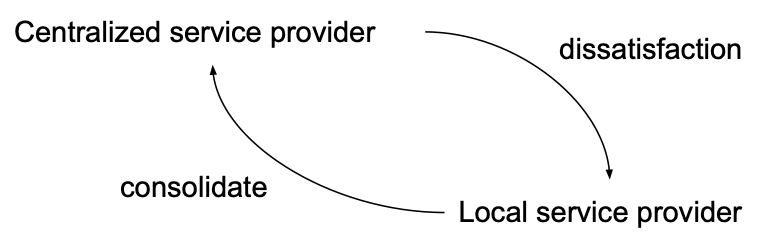
\includegraphics[width=0.8\textwidth]{images/dilemma_centralization-vs-distributed.pdf}
    \caption{Dipole oscillation. See Dilemma~\ref{table:dilemma-org-central-vs-distributed}. Migrating to the opposite paradigm gives people in charge a chance to show their responsiveness to the needs of participants. The rate of oscillation is a measure of institutional memory half-life.}
    \label{fig:central-vs-distributed}
\end{figure}

%  explanation of context for dilemma
Bureaucratic organizations are comprised of teams that provide services to other members of the organization and to subjects. A centralized approach improves efficiency through less redundancy, but also can decrease responsiveness.  
Grove~\cite{1995_Grove} calls the centralized model functional teams.

% How does this relate directly to bureaucracy as defined as shared resource management policymaking?
%The \hyperref[table:dilemma-org-central-vs-distributed]{Dilemma of Centralization of Services}
% How does this effect your relationships with other bureaucrats?
%The \hyperref[table:dilemma-org-central-vs-distributed]{Dilemma of Centralization of Services}
% Are the incentive structures aligned to support one direction or the other?

Centralization is often carried out for the purposes of cost efficiency. The cost savings are due to de-duplication and having less slack. Both of those ``savings'' are a decrease of redundancy, which has a cost when there are unexpected fluctuations in need. 

Another motive for centralization is to concentrate talent within the organization. This can have the unintentional result of silo'ing talent and isolating experts from the people they want to help.

Decentralized manifests as cross-functional teams. Do the compliance officers, financial people, or IT support staff work directly on your team locally or are they in a separate team?

%TODO -- this sentense is isolated
The rate of change between centralized and decentralized may be a function of turnover or promotion rates. \marginpar{$>>$ Speculation}

%TODO -- this sentense is isolated
A matrixed organization~\cite{1985_NASA} mixes the centralized approach and cross-functional team.

% as per chapter 8 of Andy Grove's ``high productivity management''
% When deciding between organizing functionally and organizing along business units the right answer is always the other one.


Centralization is an intentional monopolization, with a corresponding decrease in choices. 
Centralization (de-localization) can decrease the value assigned to feedback from people using the service because personal relations are devalued. 

%TODO -- this sentense is isolated
The weaker feedback, lack of redundancy, and decreased emphasis on relationships motivate the creation of local services. 


\begin{center}
\begin{table}[H] % ht
\begin{tabular}{ | m{\dilemmatablewidth}| m{\dilemmatablewidth} | } 
  \hline
  \textbf{Redundant services in a market.} &
  \textbf{Monopoly service provider.} \\
  \hline
  \textit{Description}: Using a market model within the organization. &
  \textit{Description}:  \\  
  \hline
  \textit{Pros}: Enable customers to choose the best service. &
  \textit{Pros}: Efficiency of a single service. \\
  \hline
  \textit{Cons}: Redundancy. & 
  \textit{Cons}: Might not meet the needs of all customers. \\
  \hline
\end{tabular}
\caption{
\textit{Dilemma of Monopoly.}
\index{dilemma!of monopoly}
Services within an organization. See also Figure~\ref{fig:market-vs-monopoly}.
%{\tiny Tag: Design of organization.}
}
\label{table:dilemma-org-market-vs-monopoly}
%GV     "dilemma-org-market-vs-monopoly" [label="redundant services vs monopoly", shape="box"];
%GV     "dilemma-org-market-vs-monopoly" -> "monopoly";
\end{table}
\end{center}


\begin{figure}[H] % ht
    \centering
    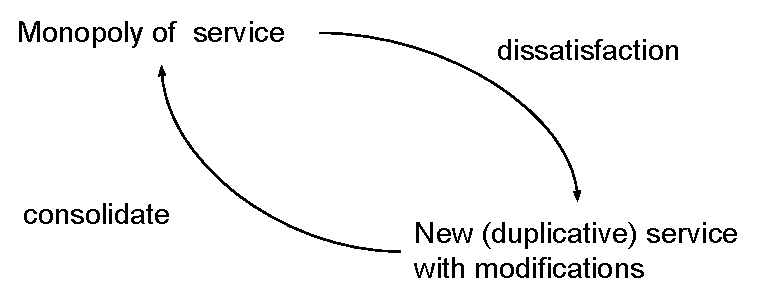
\includegraphics[width=0.8\textwidth]{images/dilemma_market_vs_monopoly.pdf}
    \caption{Dipole oscillation: solution A exists but doesn't meet my needs. Rather than tweak A, re-invent solution B. B mostly overlaps with A but has independent development and support. See also Dilemma~\ref{table:dilemma-org-market-vs-monopoly}.}
    \label{fig:market-vs-monopoly}
\end{figure}

% explanation of context for dilemma
The \hyperref[table:dilemma-org-market-vs-monopoly]{Dilemma of Monopoly} is similar to the \hyperref[table:dilemma-org-central-vs-distributed]{Dilemma of Centralization of Services}, in that both seem initially to be dipole oscillations. The centralization of services can be addressed by a matrixed organization, while an approximation of that concept for services would be federation. 

% How does this relate directly to bureaucracy as defined as shared resource management policymaking?
The \hyperref[table:dilemma-org-market-vs-monopoly]{Dilemma of Monopoly} is a label for the conflict of interest between minimizing redundancy and customizing solutions. Services tailored to the needs of a bureaucrat or subject mean that someone else with different needs will want a different solution. 

% How does this effect your relationships with other bureaucrats?
%The \hyperref[table:dilemma-org-market-vs-monopoly]{Dilemma of Monopoly}

% Are the incentive structures aligned to support one direction or the other?
The default direction for a bureaucratic organization is toward centralization and monopoly because that seems more efficient. At the same time, individual bureaucrats observe local challenges and invent solutions relevant to their needs.


\ \\

\begin{center}
\begin{table}[H] % ht
\begin{tabular}{ | m{\dilemmatablewidth}| m{\dilemmatablewidth} | } 
  \hline
  \textbf{Decision-making lower in a hierarchy.} &
  \textbf{Decision-making higher in a hierarchy.} \\
  \hline
  \textit{Description}: Push decisions down to empower employees. &
  \textit{Description}: Escalate every decision to management. \\  
  \hline
  \textit{Pros}: Better information. &
  \textit{Pros}: Better scope. \\
  \hline
  \textit{Cons}: More inconsistency. & 
  \textit{Cons}: Decision-maker has less skin in the game and may be less well-informed. Employees are disempowered. \\
  \hline
\end{tabular}
\caption{
\textit{Dilemma of Decision Height.}
\index{dilemma!of decision height}
Where decisions get made in a hierarchical organization.
%{\tiny Tag: Design of organization.}
}
\label{table:dilemma-org-decisions-low-vs-high}
%GV     "dilemma-org-decisions-low-vs-high" [label="decision-making high or low", shape="box"];
%GV     "dilemma-org-decisions-low-vs-high" -> "decisions";
\end{table}
\end{center}

% explanation of context for dilemma
Bureaucrats with direct exposure to a challenge and the ramifications are better positioned to make decisions. As Marquet~\cite{2013_Marquet} points out, pushing decisions down improves the sense of ownership. However, people directly working on a challenge may lack a holistic perspective held by bureaucrats higher in the chain of command. 

% How does this relate directly to bureaucracy as defined as shared resource management policymaking?
The \hyperref[table:dilemma-org-decisions-low-vs-high]{Dilemma of Decision Height} indicates that no individual is ideally positioned to make decisions. Bureaucracy involves distributed decision-making because no member has all the relevant information. The coordination of distributed knowledge is a remedy that requires ongoing investment.

% How does this effect your relationships with other bureaucrats?
The \hyperref[table:dilemma-org-decisions-low-vs-high]{Dilemma of Decision height} indicates that relationships up and down the chain of command are necessary. Low-level bureaucrats need to understand the holistic perspective, and bureaucrats at the top of the organization need to understand the ramifications of their decisions.

% Are the incentive structures aligned to support one direction or the other?
Relationships rarely span the chain of command, and bureaucrats make decisions based on locally accessible information and personal experience. 



\ \\

\textit{Trilemma}: \textbf{Do you support the cutting edge, most of the middle, or the laggards?}\\
\index{trilemma!cutting edge, middle, laggards}
For any given aspect of bureaucracy there is a \href{https://en.wikipedia.org/wiki/Normal_distribution}{bell curve} 
\index{Wikipedia!normal distribution@\href{https://en.wikipedia.org/wiki/Normal_distribution}{Normal distribution}}
of skills and interests of bureaucrats. In your role as a bureaucrat you face a choice: find and collaborate with and enable the best and brightest, or aim your efforts at the massive mediocre middle (most bureaucrats), or try to get the dumbest bureaucrats up to speed? 

Trying to escape the trilemma by claiming that you treat everyone equally means you are disregarding the needs of the tail of the distribution. 

\ \\

% https://graphthinking.blogspot.com/2021/12/hierarchical-organization-trilemma.html
\textit{Trilemma}: \textbf{Do you work for your team, your manager, or yourself?} \\
\index{trilemma!team, manager, yourself}
Being a member of a team that operates within a hierarchy is tough. One reason is the question of who you are working for. The trilemma is whether you work for yourself, work for your supervisor, or work for your team.  Ideally, you can find ways to do all three, but that is not always the case. 

Members of the team should work collaboratively, but there is a potential counter-force: accountability to the supervisor. Because each team member is accountable to their supervisor(s), that motivates the action of the individual. The team does not have autonomy -- they are accountable to the boss.

In the approach ``team members are directed by their supervisor," the synergy of the team is neglected and the supervisor becomes a bottleneck (for decision-making and for creativity and for planning).

The third approach is for a person to ignore their team and their supervisor. This might enable quicker progress, at the risk of going in an unhelpful direction or not leveraging the skills of coworkers. 

\ \\

\textit{Trilemma}:
\textbf{Seek less budget, same, or larger budget.} 
\index{trilemma!less, same, or larger budget}
Less budget is needed if you improve efficiency, but then the proportional power within the organization is decreased. A larger budget may be due to inefficiency or growth. Keeping the same budget indicates no promotions are relevant (although a steady state could result from a combination of growth and improved efficiency). 

\ \\

A trilemma applicable to many situations is that options are \textbf{fast, inexpensive, good; choose two}. 
\index{trilemma!fast, inexpensive, good}
(This is the \href{https://en.wikipedia.org/wiki/Project_management_triangle}{Project management triangle}.) 
\index{Wikipedia!project management triangle@\href{https://en.wikipedia.org/wiki/Project_management_triangle}{Project management triangle}}
\\
\index{folk wisdom!project management triangle@\href{https://en.wikipedia.org/wiki/Project_management_triangle}{Project management triangle}}
In other words, the options are
\begin{itemize}
    \item Good and fast is expensive (i.e., requires lots of resources).
    \item Good and inexpensive takes a long time (i.e., find a clever solution).
    \item Fast and inexpensive will be low quality.
\end{itemize}

\subsection*{Dilemmas Raised by Subjects of Bureaucracy\label{sec:subjects-dilemmas}}

%GV } // end org
%GV subgraph cluster_subject {
%GV    label = "subject dilemmas";

Each subject of bureaucracy views themselves as logical, self-consistent, and erudite. In practice, the bureaucrat serving subjects encounters conflicting statements. 

\begin{center}
\begin{table}[H] % ht
\begin{tabular}{ | m{\dilemmatablewidth}| m{\dilemmatablewidth} | } 
  \hline
  \textbf{Subject asks, ``Why do I have to fill out this form?''} &
  \textbf{Subject asks, ``Why aren't you catching more cheaters and fraudsters?''} \\
%  \hline
%  \textit{Description}:  & 
%  \textit{Description}:  \\
%  \hline
%  \textit{Pros}: . & 
%  \textit{Pros}: . \\
  \hline
  \textit{Cons}: Filling out forms is burdensome for the subject and the bureaucrat. & 
  \textit{Cons}: To detect problems and identify risks, information is needed. \\
  \hline
\end{tabular}
\caption{\textit{Dilemma of Forms}: no one likes paperwork or letting cheaters cheat. The cost of protecting scarce resources is felt by everyone.
}
\label{table:dilemma-subject-forms}
%GV     "dilemma-subject-forms" [label="burden of forms", shape="box"];
%GV     "dilemma-subject-forms" -> "forms";
\end{table}
\end{center}

% explanation of context for dilemma
Subjects of bureaucracy expect efficiency. While that's reasonable, the nuances include minimizing the burden of interaction while also making sure the shared resource managed by bureaucrats isn't misallocated to malicious or unworthy recipients. 

The 
\hyperref[table:dilemma-subject-forms]{Dilemma of Forms}
is the subject's experience of the bureaucrat's 
\hyperref[table:dilemma-personal-single-bit-decision]{Dilemma of Redundant Data for Decisions}.

% How does this relate directly to bureaucracy as defined as shared resource management policymaking?
%
% How does this effect your relationships with other bureaucrats?
As a result of the \hyperref[table:dilemma-subject-forms]{Dilemma of Forms}, bureaucrats are unable to satisfy the desire of subjects to have efficient bureaucracy. 

% Are the incentive structures aligned to support one direction or the other?


\begin{center}
\begin{table}[H] % ht
\begin{tabular}{ | m{\dilemmatablewidth}| m{\dilemmatablewidth} | } 
  \hline
  \textbf{Subjects desire consistency across situations.} &
  \textbf{Subjects seek exceptions for their specific situation.} \\
  \hline
  \textit{Description}: Predictability allows for planning. & 
  \textit{Description}: I am unique. \\
%  \hline
%  \textit{Cons}: . & 
%  \textit{Cons}: . \\
  \hline
\end{tabular}
\caption{\textit{Dilemma of Consistency.}
Consistency is seen as fairness, when in fact consistency can ignore critical differences. %Consistency is desirable for enabling predictability.
}
\label{table:dilemma-subject-consistency-per-situation}
%GV     "dilemma-subject-consistency-per-situation" [label="consistency vs exceptions", shape="box"];
%GV     "dilemma-subject-consistency-per-situation" -> "consistency";
%GV     "dilemma-subject-consistency-per-situation" -> "exception";
\end{table}
\end{center}

% explanation of context for dilemma
The origin of the \hyperref[table:dilemma-subject-consistency-per-situation]{Dilemma of Consistency} is based in narcissism on the part of subjects. ``I am uniquely special and no one else is.''  

% How does this relate directly to bureaucracy as defined as shared resource management policymaking?
%T
% How does this effect your relationships with other bureaucrats?
%The \hyperref[table:dilemma-subject-consistency-per-situation]{Dilemma of Consistency}
% Are the incentive structures aligned to support one direction or the other?
Bureaucrats seek consistency in the application of policies as a defensible story justifying the allocation of shared resources. A complicating factor is whether you think of fairness as equality (consistency means everything is the same) or equity (consistency accounts for differences). 

As with the \hyperref[table:dilemma-subject-forms]{Dilemma of Forms}, the consequence of the \hyperref[table:dilemma-subject-consistency-per-situation]{Dilemma of Consistency} is that subjects will usually be unhappy with bureaucracy. Your Process Empathy extends to how subjects view the bureaucracy you are part of.

\begin{center}
\begin{table}[H] % ht
\begin{tabular}{ | m{\dilemmatablewidth}| m{\dilemmatablewidth} | } 
  \hline
  \textbf{Subjects seek clearly defined rules.} &
  \textbf{Subjects seek flexibility in application of rules.} \\
  \hline
  \textit{Description}: Rules are seen as enabling fairness, when in fact rules can perpetuate inequality. Rules (assuming uniform enforcement) are also seen as enabling predictability. & 
  \textit{Description}: Subject may expect their status in the community or their relationship with the bureaucrat enables exceptions. \\
%  \hline
%  \textit{Pros}: . & 
%  \textit{Pros}: . \\
%  \hline
%  \textit{Cons}: . & 
%  \textit{Cons}: . \\
  \hline
\end{tabular}
\caption{\textit{Dilemma of Flexible Rules.}
}
\label{table:dilemma-subject-flexibility}
%GV     "dilemma-subject-flexibility" [label="clear rules vs flexiblity", shape="box"];
%GV     "dilemma-subject-flexibility" -> "flexibility";
\end{table}
\end{center}

%  explanation of context for dilemma
The application of policy by bureaucrats is subjective. Relying on rules to be deterministic misses the relevance of human interpretation. Predictability of rulings helps bureaucrats and subjects.

% How does this relate directly to bureaucracy as defined as shared resource management policymaking?
% How does this effect your relationships with other bureaucrats?
As with all other dilemmas, the \hyperref[table:dilemma-subject-flexibility]{Dilemma of Flexible Rules} is enacted to various degrees by different bureaucrats, resulting in non-uniform outcomes for subjects. Your relationship with the deciding bureaucrat matters. Information you provide and arguments you make sway the decider. 

% Are the incentive structures aligned to support one direction or the other?
The bias for bureaucrats faced with the \hyperref[table:dilemma-subject-flexibility]{Dilemma of Flexible Rules} is to appear consistent across decisions. The appearance of inconsistent policy application is harmful to the reputation of the bureaucrat and the organization.

\begin{center}
\begin{table}[H] % ht
\begin{tabular}{ | m{\dilemmatablewidth}| m{\dilemmatablewidth} | } 
  \hline
  \textbf{Subject wants transparency.} &
  \textbf{Subject wants low cost (free).} \\
  \hline
  \textit{Description}: Transparency requires collection and reporting of data. & 
  \textit{Description}: Access to shared resources shouldn't be costly. \\
%  \hline
%  \textit{Pros}: . & 
%  \textit{Pros}: . \\
%  \hline
%  \textit{Cons}: . & 
%  \textit{Cons}: . \\
  \hline
\end{tabular}
\caption{\textit{Dilemma of Transparency.}
Transparency has a cost.
}
\label{table:dilemma-subject-transparency}
%GV     "dilemma-subject-transparency" [label="transparency vs low cost", shape="box"];
%GV     "dilemma-subject-transparency" -> "transparency";
\end{table}
\end{center}

% explanation of context for dilemma
Whenever there is a desire for lower cost and some feature, there is a conflict of interest with the costly feature. Bureaucrats make subjective decisions, so transparency helps other people understand the reasoning behind outcomes. Transparency is not free, so a dilemma occurs. 

% How does this relate directly to bureaucracy as defined as shared resource management policymaking?
%The \hyperref[table:dilemma-subject-transparency]{Dilemma of transparency}

% How does this effect your relationships with other bureaucrats?
The \hyperref[table:dilemma-subject-transparency]{Dilemma of Transparency} depends on your role. If you are a decision-maker or data owner, you do not gain immediate value from justifying decisions or sharing data. You pay a cost to provide transparency, both reputational (your mistakes become visible) and financial (for hosting data, time spent publishing). There are potential benefits to transparency -- improved trust in relationships, subjects detecting and reporting mistakes. 

% Are the incentive structures aligned to support one direction or the other?
An incumbent bureaucrat defaults to no transparency. If subjects want to dispute decisions they benefit from having information about how the policy was applied. If the subject is willing to pay the cost for the data, then the decision-maker has to do extra work to make data available.


\subsubsection*{Consequences of the Dilemma-based Framing}

There are many dilemmas listed above but the list is not comprehensive. The point of having a detailed list rather than just a few is to illustrate the nuance and complexity of bureaucracy. 

%In light of the dilemmas, what course of action?

In practice, most bureaucrats do not choose an optimization strategy, then decide how to respond to all 60+ dilemmas.
Nor do bureaucrats talk with their fellow bureaucrats about how to respond as an organization to all 60 dilemmas.
Bureaucrats decide when forced to respond by circumstances after having deferred as long as possible. Early decisions are premature and have less information.

Decisions regarding how to respond to a dilemma are not made in isolation - one decision alters the options available for other dilemmas. The ability to project potential consequences depends on you understanding the reaction of peers, subordinates, and supervisors you depend on. Your decisions create constraints and opportunities for them.



A bureaucrat aiming to avoid dilemmas may respond by deferring to someone higher in the hierarchy to decide and coordinate. While fewer people making decisions would improve consistency, this would be \href{https://en.wikipedia.org/wiki/Micromanagement}{micromanagement}. 
\index{Wikipedia!micromanagement@\href{https://en.wikipedia.org/wiki/Micromanagement}{micromanagement}}
The people in the hierarchy above the person facing the choice don't have exposure to the problem. Choices are delegated to leverage expertise. 

\ \\

When you are facing these dilemmas and trilemmas
\marginpar{$>>$ Actionable Advice} 
\index{actionable advice}%
there are constructive responses that can improve your effectiveness. Improvement helps your results, your reputation, and the organization. 
\begin{itemize}
    \item Collect quantitative data for each variable. Quantitative arguments can augment qualitative stories. 
    \item Construct the Pareto frontier to identify non-optimal choices that can be eliminated.
    \item Instead of assessing variables in isolation, assess consequences in the context of workflows and effects on stakeholders.
    \item Discuss subjective decisions with stakeholders so that potential disagreements can be negotiated instead of creating friction.
\end{itemize}
 


Even if each bureaucrat were to consider the same dilemmas (which doesn't necessarily happen), not everyone makes the same selection. This is a source of friction in an organization. The next section expands on the  challenges inherent to bureaucracy. 

%GV } // end subject subgraph
%GV } // end digraph G